%-----------------------------------------------
%  Engineer's & Master's Thesis Template
%  Copyleft by Artur M. Brodzki & Piotr Woźniak
%  Warsaw University of Technology, 2019-2022
%-----------------------------------------------

\documentclass[
    bindingoffset=5mm,  % Binding offset
    footnoteindent=3mm, % Footnote indent
    hyphenation=false    % Hyphenation turn on/off
]{src/wut-thesis}

\graphicspath{{tex/img/}} % Katalog z obrazkami.
\addbibresource{bibliografia.bib} % Plik .bib z bibliografią

% Pakiety dodatkowe
\usepackage{tikz}
\usetikzlibrary{shapes.geometric, arrows.meta, positioning, calc}

\facultyeiti    % Wydział Elektroniki i Technik Informacyjnych
\MasterThesis % Praca magisterska
\langpol % Praca w języku polskim

\begin{document}

%------------------
% Strona tytułowa
%------------------
\instytut{Automatyki i Informatyki Stosowanej}
\kierunek{Informatyka}
\specjalnosc{Systemy Internetowe Wspomagania Zarządzania}
\title{
    Analiza efektywności lokalnych i chmurowych modeli AI \\
    do generowania opisów obrazów w aplikacjach mobilnych
}
% Title in English for English theses
% In English theses, you may remove this command
\engtitle{
    Effectiveness analysis of local and cloud AI models \\
    for image captioning in mobile applications
}

\author{Dominik Baczyński}
\album{300475}
\promotor{dr inż. Piotr Bobiński}
\date{\the\year}
\maketitle

%-------------------------------------
% Streszczenie po polsku dla \langpol
% English abstract if \langeng is set
%-------------------------------------
\cleardoublepage % Zaczynamy od nieparzystej strony
\abstract 
Praca podejmuje się problemu doboru strategii wdrażania modeli sztucznej inteligencji (AI) do generowania opisów obrazów w aplikacjach mobilnych
poprzez analizę efektywności wybranych rozwiązań lokalnych i chmurowych. 
Badania opierają się na eksperymentach porównawczych w dwóch komplementarnych wymiarach- wydajnościowym i jakościowym.
W celu realizacji badań opracowano dedykowaną platformę testową dla systemu Android umożliwiającą integrację różnych modeli sztucznej inteligencji poprzez zunifikowany, niezależny od 
implementacji, interfejs oraz automatyzacje procesu pomiarowego, w tym rejestrację metryk wydajnościowych w czasie inferencji.
Architektura platformy wykorzystuje ONNX Runtime jako silnik inferencji dla modeli lokalnych oraz REST API dla integracji z usługami chmurowymi.
Eksperymenty przeprowadzono na reprezentatywnym zbiorze danych obrazów z opisami referencyjnymi, wykorzystując lokalne modele AI uruchamiane na urządzeniu mobilnym
oraz modele chmurowe udostępniane przez zewnętrznych dostawców poprzez interfejsy API.
Każdy model został poddany wielokrotnym iteracjom pomiarowym z fazą rozgrzewkową, zapewniając wiarygodność statystyczną zebranych danych.
Zebrane w trakcie badań dane obejmują szczegółowe metryki wydajnościowe obejmujące czasy odpowiedzi, zużycie zasobów systemowych i 
koszty operacyjne oraz jakościowe generowanych opisów, ocenianych za pomocą standardowych algorytmów z dziedziny przetwarzania języka naturalnego.
Dane te stanowią podstawę do wieloaspektowej analizy porównawczej efektywności badanych strategii wdrożeniowych, umożliwiając sformułowanie wniosków
i rekomendacji dotyczących doboru optymalnego podejścia do implementacji modeli sztucznej inteligencji w zadaniu generowania opisów obrazów w aplikacjach mobilnych.
Głównym wnioskiem przeprowadzonych badań jest stwierdzenie, że specjalizacja modelu do konkretnego zadania image captioning'u ma większe znaczenie 
dla osiąganych wyników wydajnościowych i jakościowych niż sama strategia wdrożeniowa, co fundamentalnie zmienia perspektywę na problem wyboru 
między rozwiązaniami lokalnymi a chmurowymi.

\keywords sztuczna inteligencja, generowanie opisów obrazów, image captioning, aplikacje mobilne, modele lokalne, modele chmurowe, wydajność, Android, ONNX

%----------------------------------------
% Streszczenie po angielsku dla \langpol
% Polish abstract if \langeng is set
%----------------------------------------
\clearpage
\secondabstract 
This thesis addresses the problem of selecting deployment strategies for artificial intelligence (AI) models for image captioning in mobile applications
through the analysis of the effectiveness of selected local and cloud solutions.
The research is based on comparative experiments in two complementary dimensions - performance and quality.
To conduct the research, a dedicated testing platform for the Android system was developed, enabling the integration of various artificial intelligence models through a unified, implementation-independent 
interface and automation of the measurement process, including the recording of performance metrics during inference.
The platform architecture utilizes ONNX Runtime as the inference engine for local models and REST API for integration with cloud services.
The experiments were conducted on a representative dataset of images with reference captions, using local AI models running on a mobile device,
and cloud models provided by external vendors through API interfaces.
Each model was subjected to multiple measurement iterations with a warm-up phase, ensuring statistical reliability of the collected data.
The data collected during the research includes detailed performance metrics covering response times, system resource consumption, and 
operational costs, as well as quality metrics of generated captions, evaluated using standard algorithms from the field of natural language processing.
This data forms the basis for a multi-faceted comparative analysis of the effectiveness of the studied deployment strategies, enabling the formulation of conclusions
and recommendations regarding the selection of the optimal approach to implementing artificial intelligence models for image captioning tasks in mobile applications.
The main conclusion of the conducted research is that model specialization for the specific task of image captioning has greater significance 
for achieved performance and quality results than the deployment strategy itself, which fundamentally changes the perspective on the choice 
between local and cloud solutions. 
\secondkeywords artificial intelligence, image captioning, mobile applications, local models, cloud models, performance, Android, ONNX

\pagestyle{plain}

%--------------
% Spis treści
%--------------
\cleardoublepage % Zaczynamy od nieparzystej strony
\tableofcontents

%------------
% Rozdziały
%------------
\cleardoublepage % Zaczynamy od nieparzystej strony
\pagestyle{headings}

\newpage % Rozdziały zaczynamy od nowej strony.
\section*{Cel Pracy} \label{ss:Cel Pracy}

\noindent
Dynamiczny rozwój technologii oraz systemów sztucznej inteligencji umożliwił
realizację zaawansowanych i skomplikowanych obliczeniowo zadań bezpośrednio na urządzeniach mobilnych.
Postęp w architekturze modeli, metodach kompresji oraz wydajności układów (CPU/NPU) sprawił,
że aplikacje korzystające z AI stały się powszechne w środowisku mobilnym.
Równolegle wielcy dostawcy usług chmurowych udostępniają najnowocześniejsze modele AI
oferujące zaawansowane możliwości o niespotykanej wcześniej jakości i skali.
Rozwiązania te niosą jednak ze sobą zależność od zewnętrznej infrastruktury oraz wiążą się
z kwestiami prywatności, bezpieczeństwa i opłat subskrypcyjnych.

Na tym tle szczególne znaczenie zyskuje kwestia automatycznego generowania opisów obrazów 
(image captioning), łączącej zaawansowane przetwarzanie obrazu z generowaniem języka naturalnego.
Technologia ta znajduje zastosowanie w wielu aspektach, od wsparcia osób z dysfunkcją wzroku,
przez automatyczną kategoryzację treści, aż po integrację z asystentami głosowymi.


W obliczu tych możliwości twórcy aplikacji mobilnych stają przed dylematem wyboru
między wdrażaniem lokalnych modeli sztucznej inteligencji a integracją z usługami chmurowych dostawców.

Celem niniejszej pracy jest przeprowadzenie kompleksowej analizy porównawczej modeli działających 
w warunkach lokalnych oraz chmurowych w kontekście generowania opisów obrazów na urządzeniach 
z systemem Android. Badanie obejmuje porównanie trzech modeli lokalnych uruchamianych przez środowisko
ONNX Runtime (Florence-2, ViT-GPT2, BLIP) oraz trzech usług chmurowych udostępnianych przez interfejs
API (OpenAI GPT-4o mini, Azure Computer Vision, Google Gemini 2.5 Flash Lite).

Analiza efektywności poszczególnych modeli opiera się na dwóch komplementarnych aspektach:
metrykach wydajnościowych (czas generowania odpowiedzi, zużycie pamięci RAM, pobór energii, koszty wywołań API)
oraz metrykach jakościowych (poprawność generowanych opisów mierzona wskaźnikami CIDEr, SPICE, METEOR, BLEU).
Zebrane w ten sposób dane posłużą do sformułowania popartych empirycznie rekomendacji doboru rozwiązań
sztucznej inteligencji w zależności od przeznaczenia projektowanej aplikacji mobilnej.

Do realizacji powyższych celów zaprojektowano i zaimplementowano platformę badawczą CaptionLab, która
umożliwia prowadzenie badań, zbieranie metryk oraz zautomatyzowane testy na dużych zbiorach danych.
Architektura platformy badawczej została opracowana z myślą o elastyczności i rozszerzalności
dzięki jednolitemu podejściu do implementacji poszczególnych modeli w formie osobnych providerów.

Ostatecznie praca dostarcza nie tylko analityczną wiedzę odnośnie strategii wdrażania systemów 
sztucznej inteligencji w środowisku mobilnym, ale także funkcjonalną platformę badawczą, która
może służyć jako fundament dla dalszych badań lub jako funkcjonalne narzędzie przy podejmowaniu
decyzji architektonicznych w projektowaniu aplikacji mobilnych.



\newpage
\section{Wstęp}\label{s:Wstep}

\noindent
Systemy sztucznej inteligencji w ostatnich latach przeszły znaczną ewolucję od naukowych koncepcji
do powszechnie wykorzystywanych narzędzi, które zrewolucjonizowały wiele dziedzin życia i przemysłu.
AI znalazła zastosowanie i zmieniła funkcjonowanie całych sektorów gospodarki, począwszy od technologii i
rozrywki przez dziennikarstwo, kończąc na finansach czy medycynie. Według danych Presedence Research globalny rynek AI
osiągnął wartość ponad 750 miliardów USD w 2025 roku, a prognozowany dalszy wzrost, przewiduje wzrost
do prawie 3.7 bilionów USD do roku 2034 \cite{ai_market_precedence_2025}.

W spektrum zastosowań sztucznej inteligencji szczególnie wyróżnia się zadanie automatycznego generowania
opisów obrazów (image captioning) jako jedno z bardziej złożonych wyzwań łączących przetwarzanie obrazu,
kategoryzację wizualną oraz analizę kontekstu z generowaniem języka naturalnego. Systemy image captioning,
oparte na architekturach encoder-decoder \cite{show_and_tell_vinyals2015}, znajdują zastosowanie w wielu obszarach,
od wsparcia osób z dysfunkcją wzroku, przez automatyczną kategoryzację treści, aż po integrację
z asystentami głosowymi.

Rozwój technologii uczenia maszynowego umożliwił znaczący postęp w dziedzinie image captioning.
Systemy AI zyskały nowe możliwości dzięki innowacyjnym architekturom modeli oraz narzędziom
ułatwiającym deweloperom wdrażanie zaawansowanych rozwiązań.
Modele oparte na architekturze transformerów wizyjnych (Vision Transformer, ViT)
wypierały tradycyjne sieci konwolucyjne (Convolutional Neural Networks, CNN), oferując lepsze możliwości 
rozpoznawania i kwalifikacji obrazów \cite{vit_dosovitskiy2021}. Pojawienie się technologii jednolitych 
formatów modeli takich jak ONNX (Open Neural Network Exchange) umożliwiło łatwiejszą wymianę i wdrażanie 
zaawansowanych modeli AI w środowiskach o ograniczonych zasobach \cite{onnx_icsme_openja2022}, podczas gdy 
popularyzacja sieci 5G oraz rozwój chmurowego przetwarzania danych pozwoliło na korzystanie z potężnych
modeli AI poprzez interfejsy API (Application Programming Interface), eliminując potrzebę lokalnego przechowywania
i przetwarzania danych \cite{edge_computing_shi2016}.

Jednym z najbardziej dynamicznie rozwijających się obszarów zastosowań sztucznej inteligencji
są aplikacje i systemy mobilne. Współczesne urządzenia mobilne, niegdyś pełniące funkcję jedynie
narzędzi komunikacji i prostej rozrywki, dziś wyposażone są w zaawansowane układy obliczeniowe
(Neural Processing Unit, NPU) umożliwiające przetwarzanie złożonych modeli AI bezpośrednio na urządzeniach. Według raportu z 2025 roku opublikowanego przez Statista na świecie jest ponad 7 miliardów
zarejestrowanych w sieci smartfonów, co przekłada się na niemal 80\% globalnej populacji \cite{smartphone_users_2025}.
Ta masywna baza użytkowników połączona z ciągle rosnącą mocą obliczeniową układów mobilnych sprawia,
że platformy mobilne stają się kluczowym obszarem dla wdrażania rozwiązań opartych na sztucznej inteligencji.


Wybór aplikacji mobilnych jako obszaru badań nad efektywnością modeli AI jest konsekwencją szeregu specyficznych uwarunkowań środowiskowych.
Po pierwsze, urządzenia mobilne charakteryzują się ścisłymi ograniczeniami sprzętowymi, takimi jak limitowana ilość pamięci RAM, mocy obliczeniowej
czy ograniczonym źródłem zasilania. Po drugie, urządzenia funkcjonują w warunkach zmiennej jakości połączeń sieciowych, co podważa niezawodność rozwiązań 
zależnych wyłącznie od infrastruktury chmurowych dostawców. Po trzecie, kwestia prywatności i bezpieczeństwa danych użytkownika nabiera szczególnego 
znaczenia w kontekście osobistych urządzeń z dostępem do bardzo wrażliwych danych. Czynniki te powodują, że architektura systemów AI na platformach mobilnych
musi uwzględniać precyzyjny dobór rozwiązań, miejsca przetwarzania danych oraz strategii zarządzania zasobami.

W kontekście tych ograniczeń zarysowuje się istotny kompromis między podejściem lokalnym a chmurowym.
Modele uruchamiane lokalnie oferują działanie bez połączenia z siecią,
przewidywalność czasu odpowiedzi oraz silniejszą ochronę prywatności. Z drugiej strony usługi chmurowe oferują dostęp 
do najnowszych, dużych generatywnych modeli bez konieczności ich instalacji, aktualizacji czy obciążania pamięci urządzenia
kosztem zależności od sieci, kosztów subskrypcyjnych i zewnętrznego przetwarzania danych. Badania Yuyi Mao i innych wykazały,
że wybór miejsca wykonywania obliczeń (edge vs. cloud) ma istotny wpływ na opóźnienie, zużycie energii
oraz przepustowość systemu \cite{edge_vs_cloud_mao2017}. W przypadku środowiska o ograniczonych zasobach, 
chcąc jednocześnie oferować możliwie jak najlepszą jakość usługi, wybór odpowiedniego rozwiązania staje się kluczowym zadaniem projektowym dla twórców aplikacji mobilnych.


Brak kompleksowych badań porównawczych utrudnia jednak podejmowanie świadomych decyzji architektonicznych.
Niniejsza praca ma na celu wypełnienie tej luki poprzez przeprowadzenie szczegółowej analizy wydajnościowej
i jakościowej reprezentatywnych modeli lokalnych i chmurowych do generowania opisów obrazów w środowisku
mobilnym Android.


\subsection{Wymagania projektowe}\label{ss:Wymagania Projektowe}

\noindent
Głównym celem badawczym niniejszej pracy było przeprowadzenie kompleksowej analizy efektywności 
lokalnych oraz chmurowych rozwiązań sztucznej inteligencji w zadaniu generowania opisów obrazów (image captioning) 
na platformie mobilnej Android oraz sformułowanie rekomendacji doboru strategii wdrożeniowej 
w zależności od specyfiki i przeznaczenia projektowanych aplikacji mobilnych.

Kompleksowe porównanie efektywności modeli sztucznej inteligencji
w badanym kontekście wymagało
zdefiniowania problemu badawczego, doboru reprezentatywnych modeli oraz opracowania metodologii badawczej 
umożliwiającej obiektywną analizę poszczególnych modeli poprzez analizę zebranych w trakcie badań metryk.

Nim przystąpiono do realizacji głównego celu badawczego i wybrano poszczególne rozwiązania modeli sztucznej inteligencji
do analizy, należało zgłębić temat image captioning'u, poznać sam mechanizm działania, a także zrozumieć architekturę poszczególnych systemów 
dostępnych na rynku. W tym celu przeprowadzono szczegółową analizę literatury oraz dokumentacji technicznej
dotyczącej zarówno klasycznych, jak i współczesnych podejść do zadania automatycznego generowania opisów obrazów.

Na bazie tej wiedzy dokonano selekcji reprezentatywnych modeli AI różniących się architekturą, podejściem do przetwarzania danych, a także miejscem wykonywania obliczeń (lokalne vs. chmurowe). 
Wybrane modele miały pokrywać szerokie spektrum dostępnych rozwiązań,
umożliwiając w ten sposób analizę technologii o różnych podejściach i możliwościach.

Następnie, mając wyselekcjonowane rozwiązania, zaprojektowano i zaimplementowano dedykowaną platformę badawczą przystosowaną do wdrażania
i testowania różnorakich modeli AI w zadaniu image captioning'u. Platforma ta, poza wsparciem dla uruchamiania różnorodnych modeli, musiała także umożliwiać 
zbieranie precyzyjnych statystyk niezbędnych do obiektywnej analizy efektywności poszczególnych rozwiązań.

Opracowanie metodologii badawczej obejmowało zdefiniowanie zestawu metryk wydajnościowych i jakościowych, 
procedur pomiarowych oraz protokołu testowego, pozwalającego na zebranie odpowiednich danych, które w dalszej kolejności 
będą służyć do obiektywnej oceny efektywności badanych modeli AI.

Z opracowaną metodologią i sformułowanymi wymaganiami projektowymi, przystąpiono do realizacji badań, przeprowadzając serię eksperymentów
badawczych, zbierając dane dotyczące parametrów dla wybranych lokalnych i chmurowych modeli sztucznej inteligencji.

Ostatnim i zarazem kluczowym etapem była wizualizacja i interpretacja uzyskanych wyników badań, identyfikacja kompromisów między wydajnością a jakością
generowanych opisów oraz sformułowanie rekomendacji doboru strategii wdrożeniowej w zależności od specyfiki i wymagań projektowanej aplikacji mobilnej.

Wyżej sformułowane wymagania zebrano i przedstawiono w formie poszczególnych celów badawczych, których realizacja prowadzi do osiągnięcia głównego celu pracy.
Każdy z wyróżnionych niżej celów odpowiada kolejnym rozdziałom pracy, w których szczegółowo opisano podejście do realizacji i osiągnięcia poszczególnych celów.

\vspace{0.3cm}
\noindent
\textbf{Cel główny (CG):} 

Przeprowadzenie kompleksowej analizy efektywności lokalnych oraz chmurowych rozwiązań sztucznej 
inteligencji w zadaniu generowania opisów obrazów na platformie mobilnej Android 
oraz sformułowanie rekomendacji doboru strategii wdrożeniowej w zależności od specyfiki i przeznaczenia 
projektowanych aplikacji mobilnych.

\vspace{0.3cm}
\noindent
\textbf{Cele szczegółowe:}

\begin{enumerate}[leftmargin=*, label=\textbf{C\arabic*.}, itemsep=3pt]
    \item Przedstawienie teoretycznych podstaw automatycznego generowania opisów obrazów, analizy 
    architektur modeli AI stosowanych w zadaniu image captioning'u oraz identyfikacja kluczowych różnic 
    między strategiami wdrażania lokalnego i chmurowego w kontekście aplikacji mobilnych.
    
    \item Zaprojektowanie i implementacja dedykowanej platformy badawczej \textquote{CaptionLab} umożliwiającej 
    przeprowadzenie badań porównawczych modeli lokalnych i chmurowych w środowisku Android z zapewnieniem 
    precyzji pomiarów oraz powtarzalności testów.
    
    \item Opracowanie metodologii badawczej obejmującej definicję zestawu metryk wydajnościowych i jakościowych, 
    procedur pomiarowych oraz protokołów testowych pozwalających na obiektywną ocenę efektywności badanych 
    modeli AI.
    
    \item Przeprowadzenie serii eksperymentów badawczych oraz zebranie danych dotyczących parametrów wydajnościowych 
    (czas inferencji, zużycie pamięci, pobór energii, koszty operacyjne) i jakościowych (metryki CIDEr, SPICE, 
    METEOR, BLEU) dla wybranych modeli lokalnych i chmurowych.
    
    \item Interpretacja uzyskanych wyników badań, identyfikacja kompromisów między wydajnością a jakością 
    generowanych opisów oraz sformułowanie rekomendacji doboru strategii wdrożeniowej w zależności od 
    specyfiki i wymagań projektowanej aplikacji mobilnej.
\end{enumerate}

\noindent
Dla tak zdefiniowanych celów badawczych sformułowano odpowiadające im problemy badawcze,
na które niniejsza praca ma udzielić odpowiedzi. Problemy te wyznaczają główny kierunek prowadzonej
analizy oraz jasno definiują zakres prowadzonych badań.

\vspace{0.3cm}
\noindent
\textbf{Problem główny (PG):} 

Które podejście do wdrażania systemów AI generujących opisy obrazów (lokalne 
czy chmurowe) jest bardziej efektywne w środowisku mobilnym oraz jakie kryteria powinny kierować wyborem strategii wdrożeniowej?

\vspace{0.3cm}
\noindent
\textbf{Problemy szczegółowe:}

Analogicznie do dekompozycji celu głównego na cele szczegółowe problem główny został rozłożony na pięć 
problemów szczegółowych bezpośrednio odpowiadających celom szczegółowym C1-C5.

\begin{enumerate}[leftmargin=*, label=\textbf{P\arabic*.}, itemsep=3pt]
    \item Jak działa zadanie automatycznego generowania opisów obrazów,
    czym charakteryzują się poszczególne architektury modeli AI
    oraz jakie są kluczowe różnice pomiędzy strategiami wdrażania lokalnego i chmurowego?
    
    \item Jak efektywnie mierzyć i porównywać różnorodne modele AI (lokalne i chmurowe) 
    w zadaniu image captioning'u w środowisku mobilnym Android przy zapewnieniu precyzji pomiarów, 
    powtarzalności i wiarygodności eksperymentów?
    
    \item Jak opracować odpowiednią metodologię badań obejmującą wybór metryk, procedur pomiarowych 
    oraz protokołów testowych, która umożliwi obiektywną ocenę efektywności badanych modeli AI?
    
    \item Do jakich wyników prowadzą przeprowadzone eksperymenty badawcze w zakresie parametrów
    wydajnościowych i jakościowych dla wybranych lokalnych i chmurowych modeli sztucznej inteligencji?
    
    \item Jakie wnioski i rekomendacje wynikają z interpretacji zebranych danych oraz jakie 
    kompromisy i kryteria decyzyjne powinny kierować wyborem strategii wdrożeniowej 
    w zależności od specyfiki projektowanej aplikacji mobilnej?
\end{enumerate}

\noindent
Sformułowane wyżej cele oraz problemy badawcze stanowiły podstawę do wyprowadzania 
hipotez badawczych, które określają przewidywane odpowiedzi na postawione pytania badawcze. 
Hipotezy te zostały skonstruowane w oparciu o dotychczasowy stan wiedzy oraz obserwacje dotyczące kompromisów
między wydajnością a jakością w systemach uczenia maszynowego i odpowiadają kolejno postawionym problemom badawczym.

\vspace{0.3cm}
\noindent
\textbf{Hipoteza wiodąca (HG):} 

Nie istnieje uniwersalnie optymalne rozwiązanie dla wszystkich zastosowań. Modele lokalne 
charakteryzują się przewagą w zakresie ochrony prywatności, niezależności od sieci i innych dostawców, 
podczas gdy modele chmurowe oferują wyższą jakość generowanych opisów kosztem zależności od połączenia 
sieciowego i opłat operacyjnych, co implikuje konieczność doboru strategii wdrożeniowej w oparciu 
o specyficzne wymagania projektowanej aplikacji.

\vspace{0.3cm}
\noindent
\textbf{Hipotezy szczegółowe:}

\begin{enumerate}[leftmargin=*, label=\textbf{H\arabic*.}, itemsep=3pt]
    \item Architektury modeli lokalnych charakteryzują się specjalizacją i optymalizacją pod kątem ograniczonych zasobów,
    wykorzystując techniki kompresji, kwantyzacji oraz uproszczone enkodery wizyjne,
    podczas gdy modele chmurowe bazują na multimodalnych architekturach o znacznie większej pojemności,
    co przekłada się na fundamentalne różnice w strategiach wdrożeniowych.
    
    \item Efektywny pomiar i porównanie poszczególnych modeli AI wymaga dedykowanej platformy badawczej 
    implementującej ujednolicony interfejs pomiarowy, automatyzującą zbieranie metryk oraz eliminującą 
    zmienność środowiskową.
    
    \item Kompleksowa ocena efektywności modeli image captioning wymaga zdefiniowania 
    zestawu metryk wydajnościowych oraz jakościowych, 
    a także opracowania procesu testowego zapewniającego spójność i powtarzalność pomiarów pozwalających na bezpośrednie porównanie działania modeli.
    
    \item Modele lokalne charakteryzują się wyższym zużyciem pamięci RAM i energii 
    ze względu na lokalne przetwarzanie i przechowywanie wag modelu, jednak potencjalnie 
    oferują szybsze działanie, niezależne od warunków sieciowych, podczas gdy modele 
    chmurowe wykazują dłuższe czasy odpowiedzi uzależnione od opóźnień sieciowych, 
    ale zapewniają wyższe wartości metryk jakościowych.
    
    \item Interpretacja wyników prowadzi do wniosku, że modele lokalne stanowią optymalny wybór 
    dla aplikacji wymagających działania offline, niskich opóźnień, ochrony prywatności 
    oraz przewidywalnych kosztów, podczas gdy modele chmurowe są preferowane w scenariuszach 
    priorytetyzujących maksymalną jakość opisów i minimalne wymagania 
    pamięciowe aplikacji, przy akceptacji zależności sieciowej i kosztów proporcjonalnych do użytkowania.
\end{enumerate}

\noindent
Realizacja postawionych celów oraz weryfikacja sformułowanych hipotez określa strukturę logiczną pracy,
a także wyznacza kierunek prowadzonych badań. Osiągnięcie tych celów i odpowiedzi na postawione pytania badawcze
prowadzi do wyznaczenia praktycznych rekomendacji dotyczących doboru strategii wdrożeniowej systemów sztucznej inteligencji
w zadaniu image captioning'u w środowisku aplikacji mobilnych.


\subsection{Metodologia badawcza}\label{ss:Metodologia badawcza}

\noindent
W celu zrealizowania postawionych celów badawczych oraz weryfikacji sformułowanych hipotez, 
zastosowano metodologię badawczą opartą na eksperymencie porównawczym z wykorzystaniem metod ilościowych. 
Wybór tego podejścia metodologicznego wynikał z charakteru postawionego problemu badawczego, 
który wymaga obiektywnego, mierzalnego porównania dwóch odmiennych strategii wdrożeniowych 
w zadaniu generowania opisów obrazów na platformie mobilnej Android.

Wybór metody eksperymentu porównawczego był uzasadniony kilkoma kluczowymi względami. Umożliwił 
bezpośrednie zestawienie ze sobą dwóch konkurencyjnych podejść w identycznych warunkach środowiskowych, 
co wyeliminowało wpływ zewnętrznych zmiennych. Pozwolił na kontrolowanie warunków eksperymentu poprzez 
standaryzację danych wejściowych, procedur pomiarowych oraz środowiska testowego. Zapewnił również 
powtarzalność badań poprzez precyzyjne zdefiniowanie protokołu testowego, którego szczegółowy 
opis przedstawiono w rozdziale \ref{s:Metodologia badan}. \textquote{Metodologia badań}.
Porównanie obejmowało dwa komplementarne wymiary analizy. Wymiar wydajnościowy koncentrował 
się na aspektach operacyjnych działania modeli w środowisku mobilnym - czasach odpowiedzi, zużyciu 
zasobów systemowych oraz kosztach eksploatacyjnych. Wymiar jakościowy odnosił się do 
poprawności i trafności generowanych opisów obrazów mierzonej uznanymi metrykami oceny tekstu 
w języku naturalnym.

Realizacja eksperymentu porównawczego wymagała zastosowania metod ilościowych, które w przeciwieństwie 
do metod jakościowych, pozwalają na obiektywną, numeryczną ocenę badanych parametrów oraz umożliwiają 
statystyczne porównanie wyników między różnymi modelami i strategiami wdrożeniowymi. Metody ilościowe 
obejmowały pomiary bezpośrednie parametrów mierzalnych w trakcie działania modeli, takich jak 
czasy inferencji w poszczególnych fazach przetwarzania, zużycie pamięci RAM oraz 
rozmiary modeli. Zastosowano również pomiary pośrednie dotyczące kosztów operacyjnych modeli chmurowych, 
wyznaczonych na podstawie oficjalnych cenników dostawców API oraz oszacowania pobór energii urządzenia. W zakresie oceny jakości generowanych 
opisów wykorzystano uznane w literaturze metryki NLP (Natural Language Processing): CIDEr, SPICE, METEOR oraz BLEU, z których 
każda ocenia inne aspekty jakości opisu - od zgodności semantycznej, przez pokrycie pojęć, 
po płynność językową.

Takie podejście pozwoliło na obiektywną ocenę różnic między modelami lokalnymi 
a chmurowymi, statystyczne porównanie wyników oraz 
wizualizację wyników w formie wykresów i tabel ułatwiających interpretację i weryfikację postawionych hipotez
poprzez porównanie przewidywanych wartości z rzeczywistymi pomiarami, a także sformułowanie 
konkretnych, mierzalnych rekomendacji dotyczących wyboru strategii wdrożeniowej w zależności 
od przeznaczenia aplikacji.

\clearpage
\subsection{Struktura Pracy}\label{ss:Struktura Pracy}

\noindent
Wskazane cele, problemy i hipotezy badawcze w sekcji \ref{ss:Wymagania Projektowe}. \textquote{Wymagania projektowe}
zdefiniowały podział pracy na poszczególne jednostki redakcyjne, 
z których każda odpowiada realizacji kolejnych celów badawczych oraz weryfikacji postawionych hipotez.

Rozdział \ref{s:Modele}. \textit{Modele i technologie AI do generowania opisów obrazów} przedstawia szczegółowy opis teoretycznych podstaw automatycznego generowania opisów obrazów, ewolucji architektur
oraz mechanizmów działania systemów image captioning'u. Zawarto w nim także omówienie kluczowych różnic między strategiami wdrażania lokalnego i chmurowego,
a także charakterystykę wybranych modeli sztucznej inteligencji wykorzystanych w badaniach.

Szczegóły architektury i implementacji platformy badawczej zostały opisane
w rozdziale \ref{s:Aplikacja badawcza CaptionLab}. \textit{Aplikacja badawcza CaptionLab}. W ramach pracy napisany został dedykowany system badawczy 
\textquote{CaptionLab}, zdolny do przeprowadzania
testów porównawczych między różnymi modelami AI w środowisku Android, jednocześnie zbierając potrzebne 
dane do dalszej analizy. 

W rozdziale \ref{s:Metodologia badan}. \textit{Metodologia badania} przedstawiono proces projektowania i przeprowadzania 
eksperymentów badawczych, metodologię pomiarów, opis wykorzystanych w analizie metryk, a także sposób wyznaczania 
metryk jakościowych oceniających generowane opisy obrazów, na podstawie popularnych metod oceny jakości generowanego tekstu przez AI.

Wszelkie dane zebrane podczas przeprowadzania badań zostały przedstawione w rozdziale \ref{s:Wyniki badan}. \textit{Wyniki badań},
aby na ich podstawie dokonać analizy i wysnuć odpowiednią interpretację na łamach rozdziału \ref{s:Interpretacja wynikow badan}. \textit{Interpretacja wyników badań}.

Rozdział \ref{s:Podsumowanie}. \textit{Podsumowanie} zawiera końcowe wnioski z przeprowadzonych badań oraz wskazuje kierunki dalszych badań w obszarze wdrażania systemów
image captioning'u  opartych o AI na platformach mobilnych.

        
\newpage % Rozdziały zaczynamy od nowej strony.
\section{Modele i technologie AI do generowania opisów obrazów}\label{s:Modele}

\noindent
Automatyczne generowanie opisów obrazów (image captioning) stanowi jedno z fundamentalnych zadań łączących
komputerowe przetwarzanie obrazów (Computer Vision) z przetwarzaniem języka naturalnego (Natural Language Processing, NLP).
Zadanie to definiuje się jako proces przekształcania informacji wizualnej zawartej w obrazie na spójny
i semantycznie poprawny opis w języku naturalnym \cite{image_captioning_survey_hossain2019}.
Proces ten wymaga nie tylko zdolności klasyfikacji i rozpoznawania obiektów obecnych na obrazie, ale także
zrozumienia kontekstu, relacji między obiektami oraz generowania gramatycznie poprawnego opisu w docelowym języku.


Niniejszy rozdział ma na celu przedstawienie teoretycznych podstaw oraz kluczowych koncepcji jakie stoją za automatycznym generowaniem opisów obrazów.
Omówiona zostanie architektura typowych systemów image captioning, strategie wdrożeniowe z podziałem na modele lokalne i chmurowe, 
a także szczegółowy opis i uzasadnienie wyboru konkretnych modeli AI wykorzystanych w badaniach przeprowadzonych w ramach pracy.

\subsection{Architektura modeli image captioning}\label{ss:Architektura modeli}

\noindent
Tradycyjne podejścia do automatycznego generowania opisów obrazów opierały się na kombinacji metod ekstrakcji cech wizualnych z obrazów
oraz klasycznych metod generowania języka, wykorzystując ręcznie zaprojektowane deskryptory obrazu oraz 
szablonowe (template-based) bądź oparte na wyszukiwaniu (retrieval-based) metody generacji języka \cite{image_captioning_survey_hossain2019}.
Metody te jednak wymagały znacznego nakładu pracy eksperckiej w procesie projektowania cech i reguł, a ich możliwości generalizacji były znacząco ograniczone.
Wraz z rozwojem głębokiego uczenia (Deep Learning),
pojawiły się zaawansowane modele oparte na architekturach sieci neuronowych, które znacząco poprawiły
jakość generowanych opisów poprzez automatyczne uczenie się hierarchicznych reprezentacji wizualnych i językowych
bez potrzeby ręcznego projektowania cech.

Jednym z przełomów w tej dziedzinie było zastosowanie architektury enkoder–dekoder wykorzystującej sieć konwolucyjną (Convolutional Neural Network, CNN) jako enkoder 
do ekstrakcji cech z obrazu oraz rekurencyjną sieć neuronową (Recurrent Neural Network, RRN) do generowania sekwencji słów \cite{show_and_tell_vinyals2015}.
Model ten, nazywany "Show and Tell", stał się fundamentem w dalszym rozwoju systemów image captioning'u, wyznaczając nowy
złoty standard. Kolejnym przełomem było wprowadzenie mechanizmu uwagi (Attention Mechanism), który pozwala
sieciom dynamicznie skupiać się na różnych regionach obrazu podczas generowania kolejnych słów opisu \cite{attention_xu2015},
znacząco poprawiając jakość generowanych opisów.

Zmiana podejścia nastąpiła wraz z wprowadzeniem dekoderów transformerowych (Transformer-based Decoders), które zastąpiły komponenty rekurencyjne systemów.
Modele takie jak Meshed-Memory Transformer 
czy architektury wizyjno-językowe (Vision-Language Models) wykorzystujące transformery wizyjne (ViT) jako enkodery,
osiągają rezultaty przewyższające tradycyjne podejścia CNN-RNN \cite{transformer_captioning_cornia2020}.

Modele generacji opisów obrazów można podzielić na dwie główne kategorie: klasyczne modele enkoder-dekoder z mechanizmem uwagi 
oraz nowoczesne, zintegrowane modele multimodalne end-to-end.

W klasycznym ujęciu architektura systemu enkoder-dekoder z mechanizmem uwagi składa się z dwóch głównych faz: fazy ekstrakcji cech wizualnych
przez klasyczną sieć konwolucyjną, bądź bardziej złożony Vision Transformer oraz fazy generowania opisu tekstowego 
przy pomocy modelu językowego\cite{show_and_tell_vinyals2015}. Enkoder wizyjny przetwarza wejściowy obraz na sekwencję cech, 
które następnie są wykorzystywane przez dekoder językowy do generowania kolejnych tokenów opis. 
Mechanizm uwagi pozawala dekoderowi dynamicznie skupiać się na istotnych w danym kroku częściach obrazu podczas generowania każdego słowa, 
co poprawia spójność i trafność opisów. Schemat tej architektury przedstawiono na rysunku \ref{fig:encoder_decoder_architecture}.

\begin{figure}[!h]
    \centering
    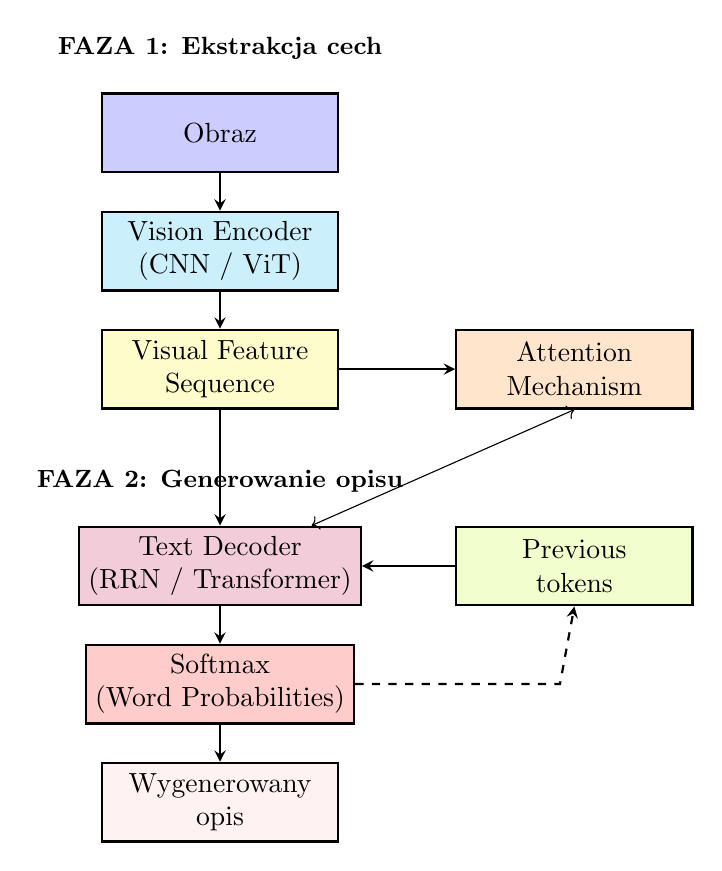
\begin{tikzpicture}[
        node distance=1.5cm,
        box/.style={rectangle, draw, thick, minimum width=3cm, minimum height=1cm, align=center},
        arrow/.style={->, thick, >=stealth}
    ]
        \node[box, fill=blue!20] (image) {Obraz};
        \node[box, fill=cyan!20, below of=image] (encoder) {Vision Encoder\\(CNN / ViT)};
        \node[box, fill=yellow!20, below of=encoder] (features) {Visual Feature\\Sequence};
        \node[box, fill=orange!20, right of=features, xshift=3cm] (attention) {Attention\\Mechanism};
        \node[box, fill=purple!20, below of=features, yshift=-1cm] (decoder) {Text Decoder\\(RRN / Transformer)};
        \node[box, fill=lime!20, right of=decoder, xshift=3cm] (prev_words) {Previous\\tokens};
        \node[box, fill=red!20, below of=decoder] (output) {Softmax\\(Word Probabilities)};
        \node[box, fill=pink!20, below of=output] (caption) {Wygenerowany\\opis};
        
        \draw[arrow] (image) -- (encoder);
        \draw[arrow] (encoder) -- (features);
        \draw[arrow] (features) -- (decoder);
        \draw[arrow] (features) -- (attention);
        \draw[<->] (attention.south) -- (decoder);
        \draw[arrow] (prev_words) -- (decoder);
        \draw[arrow] (decoder) -- (output);
        \draw[arrow] (output) -- (caption);
        \draw[arrow, dashed] (output.east) -- ++(2.6,0) -- (prev_words.south);
        
        \node[above=0.3cm of image, font=\small\bfseries] {FAZA 1: Ekstrakcja cech};
        \node[above=0.3cm of decoder, font=\small\bfseries] {FAZA 2: Generowanie opisu};
        
    \end{tikzpicture}
    \caption{Architektura systemu image captioning oparta na modelu enkoder-dekoder z mechanizmem uwagi}
    \label{fig:encoder_decoder_architecture}
\end{figure}

Współczesne podejście multimodalne dąży do integracji różnych modalności (np. obraz, tekst, audio) w ramach jednej, unifikowanej architektury end-to-end.
Zamiast sekwencyjnego przetwarzania w oddzielnych modułach enkodera i dekodera, modele te wykorzystują złożone sieci neuronowe
do przetwarzania wspólnego strumienia tokenów wizualnych i tekstowych, które są poddawane wielowarstwowej transformacji z mechanizmami uwagi krzyżowej (cross-attention)
w ramach tej samej sieci \cite{blip_li2022}. Uproszczony schemat architektury multimodalnej przedstawiono na rysunku \ref{fig:multimodal_architecture}.

\begin{figure}[!ht]
    \centering
    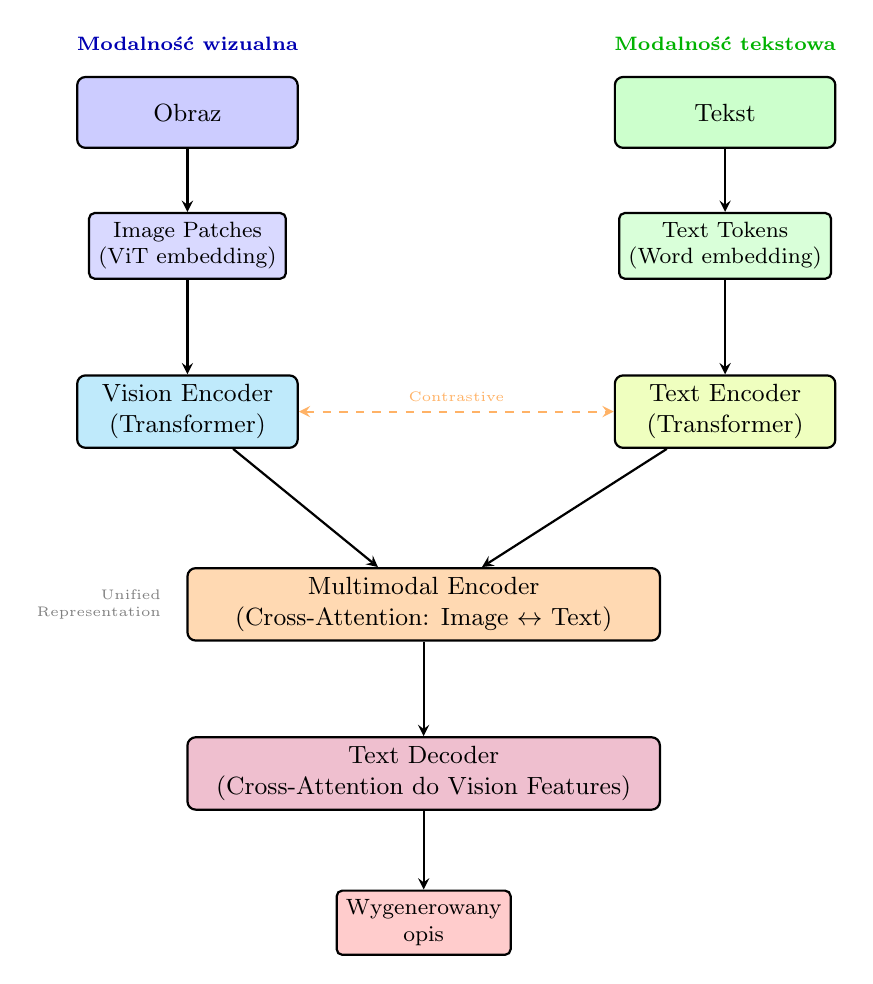
\begin{tikzpicture}[
        node distance=1.2cm and 1.5cm,
        box/.style={rectangle, draw, thick, rounded corners=3pt, minimum width=2.8cm, minimum height=0.9cm, align=center, font=\small},
        smallbox/.style={rectangle, draw, thick, rounded corners=2pt, minimum width=2cm, minimum height=0.6cm, align=center, font=\footnotesize},
        flow/.style={->, thick, >=stealth},
        biflow/.style={<->, thick, >=stealth, dashed}
    ]
        % Input layer
        \node[box, fill=blue!20] (image) {Obraz};
        \node[box, fill=green!20, right=4cm of image] (text) {Tekst};
        
        % Embedding layer
        \node[smallbox, fill=blue!15, below=0.8cm of image] (img_emb) {Image Patches\\(ViT embedding)};
        \node[smallbox, fill=green!15, below=0.8cm of text] (txt_emb) {Text Tokens\\(Word embedding)};
        
        % Encoder layer - dual stream
        \node[box, fill=cyan!25, below=1.2cm of img_emb] (vis_enc) {Vision Encoder\\(Transformer)};
        \node[box, fill=lime!25, below=1.2cm of txt_emb] (txt_enc) {Text Encoder\\(Transformer)};
        
        % Multimodal fusion
        \node[box, fill=orange!30, below=1.5cm of vis_enc, xshift=3cm, minimum width=6cm] (mm_enc) {Multimodal Encoder\\(Cross-Attention: Image $\leftrightarrow$ Text)};
        
        % Decoder
        \node[box, fill=purple!25, below=1.2cm of mm_enc, minimum width=6cm] (decoder) {Text Decoder\\(Cross-Attention do Vision Features)};
        
        % Outputs
        \node[smallbox, fill=red!20, below=1cm of decoder] (cap_out) {Wygenerowany\\opis};
        
        % Arrows
        \draw[flow] (image) -- (img_emb);
        \draw[flow] (text) -- (txt_emb);
        \draw[flow] (img_emb) -- (vis_enc);
        \draw[flow] (txt_emb) -- (txt_enc);
        \draw[flow] (vis_enc) -- (mm_enc);
        \draw[flow] (txt_enc) -- (mm_enc);
        \draw[flow] (mm_enc) -- (decoder);
        \draw[flow] (decoder) -- (cap_out);
        
        % Cross connections for contrastive
        \draw[biflow, orange!60] (vis_enc.east) -- (txt_enc.west) node[midway, above, font=\tiny] {Contrastive};
        
        % Labels
        \node[above=0.2cm of image, font=\scriptsize\bfseries, text=blue!70!black] {Modalność wizualna};
        \node[above=0.2cm of text, font=\scriptsize\bfseries, text=green!70!black] {Modalność tekstowa};
        \node[left=0.2cm of mm_enc, font=\tiny, align=right, text=gray] {Unified\\Representation};
        
    \end{tikzpicture}
    \caption{Architektura ujednoliconego modelu multimodalnego dla obrazu i tekstu.}
    \label{fig:multimodal_architecture}
\end{figure}

Takie podejście do budowy modeli umożliwia bardziej efektywne wykorzystanie informacji z różnych modalności, gdyż słowa i regiony obrazu 
współuczestniczą w budowie kontekstu na każdym etapie przetwarzania. Pozwala to na głębsze zrozumienie relacji między cechami wizualnymi, a generowanym tekstem,
co przekłada się na opis obrazu, który posiada głębsze zrozumienie kontekstu sceny.

Najnowszym etapem rozwoju są wielkie modele multimodalne (Large Multimodal Models, LMMs), które są bezpośrednim rozszerzeniem wielkich modeli językowych
(Large Language Models, LLMs) o zdolność przetwarzania wielomodalnych danych wejściowych, w tym obrazów, audio i wideo \cite{gpt4v_yang2023}.
Modele takie jak GPT-4 Vision oraz rodzina Gemini reprezentują paradygmat
\textquote{natively multimodal} \cite{gpt4_openai2023}, w którym wszystkie modalności są przetwarzane przez jedną zunifikowaną architekturę transformerową od samego początku procesu
treningu, w przeciwieństwie do wcześniejszych podejść łączących osobne enkodery dla różnych modalności \cite{gemini_team2023}. 

Te zaawansowane LMM'y, dostępne głównie jako usługi chmurowe przez API dostawców (OpenAI API, Google Vertex AI),
oferują bezprecedensowe możliwości w zakresie rozumienia i generowania opisów obrazów, łącząc bogate reprezentacje wizualne
z zaawansowanymi zdolnościami rozumowania i generowania języka naturalnego charakterystycznymi dla wielkich modeli językowych.

\subsection{Strategia wdrożenia modeli sztucznej inteligencji}\label{ss:Strategia wdrozenia}
\noindent
W środowisku mobilnym istnieją dwie główne strategie wdrażania rozwiązań sztucznej inteligencji. Pierwsza z nich to implementacja modeli lokalnych, które są zoptymalizowane do 
działania bezpośrednio na urządzeniach mobilnych korzystając z ich zasobów. Druga obejmuje wykorzystanie gotowych rozwiązań AI dostępnych jako usługi chmurowe (AI-as-a-Service) 
i integrację ich poprzez internetowe API.

Implementacja modeli sztucznej inteligencji natywnie na urządzeniu mobilnym wymaga zastosowania dedykowanych silników inferencji (Inference Runtime) 
oraz formatów modeli dostosowanych do ograniczeń sprzętowych urządzeń. Najpopularniejszymi rozwiązaniami na rynku są TensorFlow Lite (TFLite) oraz ONNX Runtime Mobile, 
które umożliwiają uruchamianie zoptymalizowanych modeli AI na zasobach urządzenia.

W celu optymalizacji modeli pod względem moblinych zastowań stosuje się różnorodne techniki kompresji i przyspieszenia inferencji, takie jak kwantyzacja (Quantization) czy
przycinanie (Pruning). Kwantyzacja polega na redukcji zapisu precyzji wag, co redukuje rozmiar modelu i przyspiesza obliczenia kosztem niewielkiej utraty dokładności \cite{tflite_quantization_krishnamoorthi2018}.

Kluczową zaletą podejścia lokalnego jest pełna niezależność od połączenia sieciowego. Dodatkowo, to podejście zapewnia silniejszą ochronę prywatności i danych
użytkownika, gdyż wszystkie dane przetwarzane są lokalnie na urządzeniu bez konieczności przesyłania ich do zewnętrznych serwerów \cite{tinyml_reddi2021}.

Ograniczenia takiej implementacji wynikają głównie z konieczności dostosowania modeli do ograniczeń sprzętowych środowiska mobilnego, co wymusza
stosowanie technik kompresji czy używania mniejszych architektur modeli, w wyniku czego modele lokalne często oferują niższą dokładność i jakość predykcji opisów.

Alternatywą jest wdrożenie AI jako usługi chmurowej poprzez integrację z API dostawców, którzy oferują dostęp do najnowocześniejszych multimodalnych modeli generatywnych 
o ogromnej mocy obliczeniowej, zdolnych do przetwarzania danych na gigantyczną skalę 
,co pozwala na uzyskanie najwyższej jakości generowanych opisów obrazów.

Wady takiego podejścia obejmują konieczność stałego połączenia sieciowego, co przekłada się na potencjalnie wyższe opóźnienia, czy brak dostępu do usługi. 
Badania Yuyi Mao i innych wskazują, że opóźnienie end-to-end w systemach chmurowych może być 3-5 razy wyższe niż w przypadku
przetwarzania lokalnego, szczególnie w warunkach słabej jakości połączenia sieciowego \cite{edge_vs_cloud_mao2017}.
Problemem są również koszty związane z wywołaniami API oraz obawy dotyczące prywatności danych.

% \vfill
\subsection{Modele lokalne wykorzystane w badaniach}\label{ss:Modele lokalne}
\noindent
Do implementacji modeli lokalnych w platformie badawczej użyto środowiska ONNX Runtime Mobile. Wybór ten podyktowany był neutralnością względem dostawcy modelu,
co pozwoliło na łatwiejszy eksport i integrację modeli o różnych architekturach w jendolitym interfejsie badawczym. Dodatkowo ONNX Runtime zapewnia wsparcie 
dla akceleracji sprzętowej wykorzystując dostępne na urządzeniu delegaty (CPU, GPU, NPU), co umożliwia przyszłe rozszerzenia bez zmian w warstwie abstrakcji.

Dobór lokalnych modeli odzwierciedla trzy generacje rozwoju podejść image captioning'u: klasyczne połączenie osobnego enkodera obrazu z dekoderem językowym (ViT-GPT2), 
nowszą ujednoliconą architekturę z podejściem enkoder-dekoder (Florence-2) oraz podejście łączące wielofunkcyjne komponenty w ramach jednego modelu (BLIP).
Taki zestaw pozwala porównać koszty obliczeń, wielkość modeli, sposób generowania opisów oraz odporność na zmianę dziedziny danych.

\subsubsection{ViT-GPT2}\label{sss:ViT-GPT2}
\noindent
Model ViT-GPT2 jest przykładem klasycznego podejścia enkoder-dekoder, łącząc Vision Transformer (ViT) jako enkoder obrazu 
z modelem językowym GPT-2 jako dekoder tekstu. W tej architekturze enkoder przetwarza wejściowy obraz na sekwencję cech w postaci 
wektorów reprezentujących różne fragmenty obrazu, które następnie dekoder wykorzystuje do generowania opisu słowo po słowie \cite{vitgpt2_blog_kumar2022}.

Model ten oferuje około 100-200 milionów parametrów w zależności od kwantyzacji, co stawia go w kategorii modeli o średniej wielkości i 
jest odpowiedni dla mobilnego środowiska. W aplikacji badawczej wykorzystano wersję modelu w formacie ONNX w kwantyzacji INT8, ze względu
na optymalizację rozmiaru i szybkości inferencji. Finalnie model ten składa się z dwóch plików, enkodera i dekodera o łącznym rozmiarze 232 MB. 
Model ten będzie stanowić punkt odniesienia do oceny nowszych architektur. 

\subsubsection{Florence-2}\label{sss:Florence-2}
\noindent
Florence-2 to zaawansowany wielozadaniowy model zdolny do realizacji zadań wizyjno-językowych, w tym generowania opisów obrazów,
detekcji obiektów, wydzielania segmentów, czy odpowiadania na pytania dotyczące obrazu \cite{florence2_xiao2024}.
Architektura modelu łączy w sobie enkoder wizyjny DaViT (Dual-Attention Vision Transformer) z modelem tekstowym BART (Bidirectional and Auto-Regressive Transformers),
przetwarzając wspólne cechy wizualne i tekstowe w standardowej strukturze enkoder-dekoder z mechanizmami uwagi krzyżowej.

Do badań wykorzystano model Florence-2-base, który najpierw został skonwertowany do formatu ONNX, jednocześnie optymalizując go do kwantyzacji 
INT8, tak aby odpowiadał on pozostałym modelom wykorzystywanych w tej pracy. Łączny rozmiar modelu po kwantyzacji wyniósł 213 MB.

\subsubsection{BLIP}\label{sss:BLIP}
\noindent
BLIP (Bootstrapping Language-Image Pre-training) to nowoczesny model wizyjno-językowy, w którym to jeden szkielet architektoniczny 
stanowi połączenie dwóch enkoderów, wizualnego i tekstowego, z dekoderem tekstowym w ramach jednolitej architektury \cite{blip_li2022}.

BLIP wyróżnia się innowacyjnym procesem treningu 
łączącym nadzorowane uczenie z automatyczną generacją i filtrowaniem syntetycznych opisów. 
Takie podejście pozwala modelowi uczyć się na dużych zbiorach danych o \textquote{zaszumionej} postaci, 
co przekłada się na lepszą generalizację.

Podobnie jak w pozostałych przypadkach w badaniach użyto wariantu skonwertowanego do formatu ONNX skwantyzowanego do INT8, 
składającego się z dwóch plików ONNX o łącznym rozmiarze 239 MB.

\subsection{Modele chmurowe wykorzystane w badaniach}\label{ss:Modele chmurowe}
\noindent
Modele chmurowe oferują dostęp do najnowocześniejszych architektur multimodalnych za pośrednictwem internetowego REST API, 
co pozwala na bezproblemową integrację z dowolną usługą. 

W badaniach wykorzystano trzy modele, reprezentujące odmienne kategorie usług: lekki uniwersalny multimodalny model ogólnego przeznaczenia (GPT-4o mini),
wyspecjalizowana usługa analizy obrazu (Azure Computer Vision) oraz ekonomiczny wariant rodziny Gemini (Gemini 2.5 Flash Lite), charakteryzujący się krótkim czasem odpowiedzi 
i efektywnością kosztową przy przetwarzaniu zapytań z obrazami. Taki dobór pozwala na ocenę kompromisu między jakością opisu, zakresem funkcji, 
kosztem przetwarzania oraz opóźnieniami zapytań sieciowych.

\subsubsection{OpenAI GPT-4o mini}\label{sss:GPT4o}
\noindent
GPT-4o mini to zoptymalizowana wersja multimodalnego modelu GPT-4o firmy OpenAI, wykorzystująca architekturę transformer natively multimodal, 
w której przetwarzanie wizualne i tekstowe jest zintegrowane od podstaw \cite{gpt4omini_openai2024}.
Jako model LLM dysponuje szeroką wiedzą ogólną oraz zdolnościami tworzenia bogatych, kontekstualnych opisów obrazów 
wykraczających poza prostą identyfikację obiektów.

Integracja odbywa się poprzez standardowe zapytania HTTPS REST API, gdzie obraz jest przesyłany 
jako załącznik w formacie base64 lub poprzez URL, a model zwraca wygenerowany opis w odpowiedzi JSON.
Czas odpowiedzi wynosi zazwyczaj 1-3 sekundy.
Model cenowy obejmuje \$0.150 za milion tokenów wejściowych oraz \$0.600 za milion tokenów wyjściowych \cite{openai_pricing2024}.

\subsubsection{Azure Computer Vision}\label{sss:Azure}
\noindent
Azure Computer Vision to wyspecjalizowana usługa analizy obrazów firmy Microsoft, zaprojektowana specjalnie do zadań przetwarzania obrazów.
Architektura opiera się na konwolucyjnych sieciach neuronowych z mechanizmami uwagi, oferując funkcje obejmujące generowanie opisów, 
wykrywanie obiektów, rozpoznawanie tekstu oraz klasyfikację treści \cite{azure_cv_docs2024}.

Integracja odbywa się poprzez Azure REST API, gdzie obrazy są przesyłane jako dane binarne lub URL.
Usługa zwraca odpowiedź JSON zawierającą opis tekstowy, wykryte obiekty, tagi oraz współczynniki pewności.
Średni czas odpowiedzi wynosi 500ms-2s.
Model cenowy obejmuje od \$1.00 do \$1.50 za 1000 transakcji \cite{azure_pricing2024}.

\subsubsection{Gemini 2.5 Flash}\label{sss:Gemini}
\noindent
Gemini 2.5 Flash to multimodalny model AI firmy Google zaprojektowany z naciskiem na szybkość i efektywność.
Wykorzystuje architekturę transformer natively multimodal, przetwarzającą dane wizualne i tekstowe wspólnie od początku treningu,
co umożliwia głębszą integrację różnych modalności \cite{gemini_team2024}.
Model obsługuje długie konteksty do 1 miliona tokenów, osiągając czas odpowiedzi 500ms-1.5s.

Dostęp odbywa się poprzez Google AI API lub z wykorzystaniem protokołu REST API. 
Model cenowy wynosi \$0.100 za milion tokenów wejściowych oraz \$0.40 za milion tokenów wyjściowych, 
co czyni go najtańszym spośród badanych rozwiązań chmurowych \cite{gemini_pricing2024}.

\subsection{Porównanie rozwiązań AI}\label{ss:Porownanie rozwiazan AI}
\noindent
Wybrane modele reprezentują różnorodne podejścia do generowania opisów obrazów, różniąc się architekturą, 
strategią wdrożenia oraz kompromisami między wydajnością a jakością. Tabela \ref{tab:models_comparison} 
przedstawia kluczowe charakterystyki wszystkich sześciu modeli wykorzystanych w badaniach.

\begin{table}[!ht]
    \centering
    \caption{Porównanie modeli lokalnych i chmurowych wykorzystanych w badaniach}
    \label{tab:models_comparison}
    \begin{tabular}{|>{\centering}m{2.2cm}|>{\centering}m{2.1cm}|>{\centering}m{2cm}|>{\centering}m{3.2cm}|>{\centering\arraybackslash}m{4cm}|}
        \hline
        \textbf{Model} & 
        \textbf{Typ} & 
        \textbf{Rozmiar / Koszt} & 
        \textbf{Architektura} & 
        \textbf{Kluczowe cechy} \\ 
        \hline\hline

        \multicolumn{5}{|c|}{\textbf{Modele lokalne (ONNX Runtime)}} \\
        \hline

        ViT-GPT2 & 
        Lokalny & 
        232 MB (INT8) & 
        ViT + GPT-2 (enkoder-dekoder) & 
        Klasyczna architektura, baseline do porównań \\
        \hline

        Florence-2 & 
        Lokalny & 
        213 MB (INT8) & 
        DaViT + BART (multi-task) & 
        Wielozadaniowy, promptowanie \\
        \hline

        BLIP & 
        Lokalny & 
        239 MB (INT8) & 
        ViT + Transformer (bootstrap) & 
        Bootstrap learning, CapFilt, kontrastywne uczenie \\
        \hline\hline

        \multicolumn{5}{|c|}{\textbf{Modele chmurowe (REST API)}} \\
        \hline

        GPT-4o mini & 
        Chmurowy & 
        \$0.15/\$0.60 za 1M tokenów & 
        Transformer (natively multimodal) & 
        LLM z wiedzą ogólną, bogate opisy, 1-3s latencja \\
        \hline

        Azure CV & 
        Chmurowy & 
        \$1.00-\$1.50 za 1k wywołań & 
        CNN + Attention (wyspecjalizowany) & 
        Dedykowany do CV, szybki (0.5-2s), pewność predykcji \\
        \hline

        Gemini 2.5 Flash & 
        Chmurowy & 
        \$0.10/\$0.40 za 1M tokenów & 
        Transformer (natively multimodal) & 
        Najtańszy, szybki (0.5-1.5s), długi kontekst (1M tokenów) \\
        \hline

    \end{tabular}
\end{table}

Modele lokalne charakteryzują się podobnym rozmiarem (213-239 MB) po kwantyzacji do INT8, 
co czyni je odpowiednimi do wdrożenia mobilnego przy zachowaniu akceptowalnej jakości. 
ViT-GPT2 stanowi punkt odniesienia jako reprezentant klasycznej architektury enkoder-dekoder, 
podczas gdy Florence-2 i BLIP reprezentują nowsze podejścia z wielozadaniowością i agregacyjym uczeniu.

Modele chmurowe oferują dostęp do znacznie większych architektur bez obciążania pamięci urządzenia, 
kosztem zależności od połączenia sieciowego i opłat za użycie. GPT-4o mini wykorzystuje szeroką wiedzę 
językową do generowania kontekstualnych opisów, Azure Computer Vision oferuje wyspecjalizowane 
przetwarzanie obrazów z krótkimi czasami odpowiedzi, a Gemini 2.5 Flash łączy niską cenę 
z szybkością, co czyni go atrakcyjnym dla aplikacji wymagających częstych zapytań.

Wybór między rozwiązaniami lokalnymi a chmurowymi sprowadza się do kompromisu między niezależnością 
od sieci i prywatnością (modele lokalne) a dostępem do najnowocześniejszych możliwości AI 
i brakiem ograniczeń pamięciowych (modele chmurowe). Przeprowadzone badania mają na celu 
empiryczną ocenę tych kompromisów w kontekście rzeczywistych metryk wydajnościowych i jakościowych.
        
% \newpage % Rozdziały zaczynamy od nowej strony.
\clearpage
\section{Aplikacja badawcza CaptionLab}\label{s:Aplikacja badawcza CaptionLab}
\noindent
W celu przeprowadzenia kompleksowych badań porównawczych wybranych modeli AI, zaprojektowano 
dedykowaną aplikację badawczą \textquote{CaptionLab} na system Android. Platforma ta, musiała umożliwiać testowanie
zarówno lokalnych oraz chmurowych modeli AI,
dostarczać odpowiednich narzędzi do zbierania danych w trakcie inferencji, a także oferować możliwość eksportu zebranych danych do dalszej analizy.

W tym rozdziale opisano architekturę systemu badawczego, jego kluczowe komponenty odpowiedzialne za generowanie opisów obrazów 
i pomiar parametrów wydajności, a także mechanizm dostarczania modeli AI, system zbierania metryk oraz moduł testów automatycznych.

\subsection{Architektura systemu}\label{ss:Architektura systemu}
\noindent
Budowa platformy \textquote{CaptionLab} opiera się na modularnej architekturze, złożonej z wyraźnie wydzielonych warstw funkcjonalnych.
System został podzielony na trzy główne warstwy: warstwę prezentacji odpowiedzialną za interfejs i interakcję z użytkownikiem,
warstwę logiki biznesowej odpowiedzialną za przeprowadzanie testów i przepływ danych oraz warstwę providerów AI implementującą 
konkretne modele sztucznej inteligencji.

Schemat architektury wysokiego poziomu przedstawiono na rysunku \ref{fig:captionlab_architecture}., który ilustruje 
najważniejsze elementy platformy, wzajemne relacje między poszczególnymi warstwami oraz przepływ danych w systemie.


\begin{figure}[!h]
    \centering
    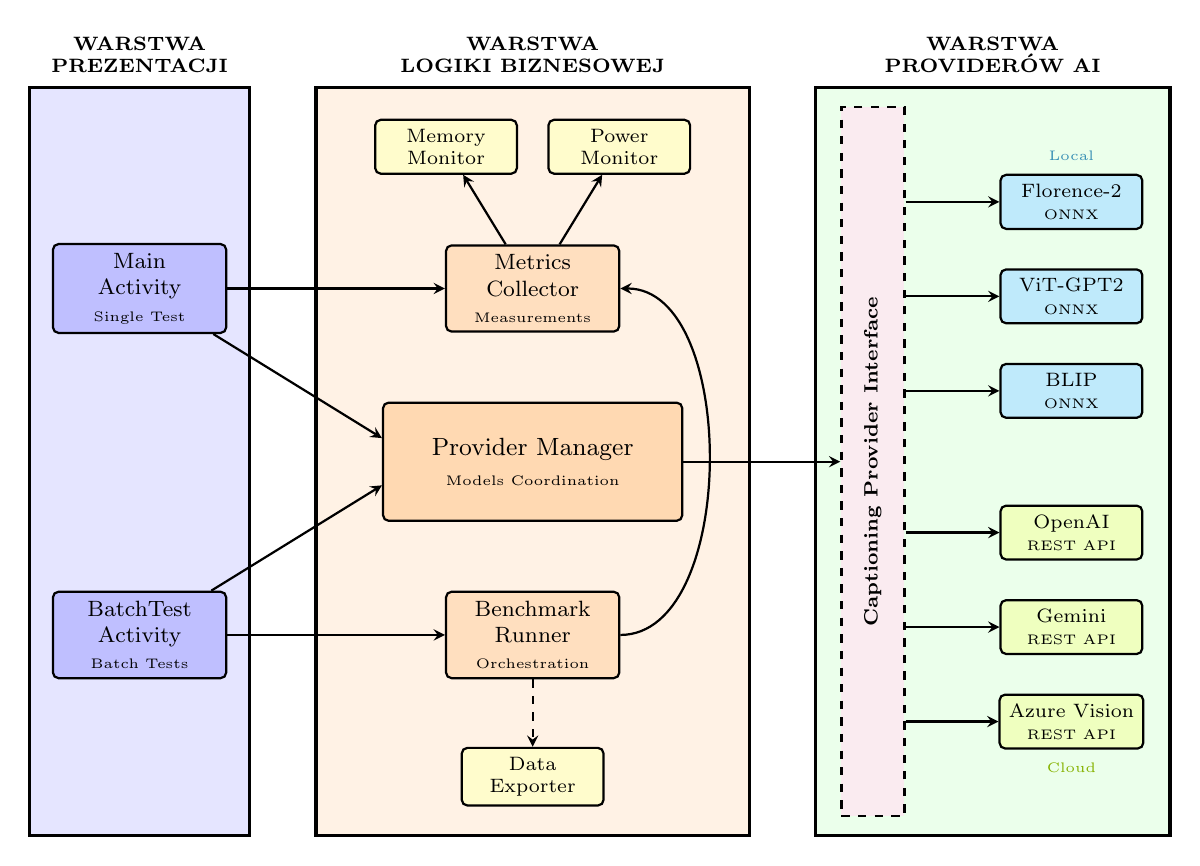
\begin{tikzpicture}[
        node distance=0.6cm,
        layer/.style={rectangle, draw=black, very thick, minimum height=9.5cm, align=center},
        component/.style={rectangle, draw, thick, rounded corners=2pt, minimum width=2.2cm, minimum height=0.8cm, align=center, font=\footnotesize},
        widecomp/.style={rectangle, draw, thick, rounded corners=2pt, minimum width=3.8cm, minimum height=1.5cm, align=center, font=\small},
        smallcomp/.style={rectangle, draw, thick, rounded corners=2pt, minimum width=1.8cm, minimum height=0.65cm, align=center, font=\scriptsize},
        interface/.style={rectangle, draw, thick, dashed, minimum height=9cm, minimum width=0.8cm, align=center},
        flow/.style={->, thick, >=stealth},
        dataflow/.style={->, thick, >=stealth, dashed}
    ]
        % WARSTWA PREZENTACJI 
        \node[layer, fill=blue!10, minimum width=2.8cm] (pres_layer) at (0,0) {};
        \node[above=0.05cm of pres_layer.north, font=\bfseries\scriptsize, align=center] {WARSTWA\\PREZENTACJI};
        
        \node[component, fill=blue!25] (main_act) at (0,2.2) {Main\\Activity\\{\tiny Single Test}};
        \node[component, fill=blue!25] (batch_act) at (0,-2.2) {BatchTest\\Activity\\{\tiny Batch Tests}};
        
        % WARSTWA LOGIKI BIZNESOWEJ
        \node[layer, fill=orange!10, minimum width=5.5cm, right=0.8cm of pres_layer] (logic_layer) {};
        \node[above=0.05cm of logic_layer.north, font=\bfseries\scriptsize, align=center] {WARSTWA\\LOGIKI BIZNESOWEJ};
        
        \node[widecomp, fill=orange!30] (provider_mgr) at ($(logic_layer)+(0,0)$) {Provider Manager\\{\tiny Models Coordination}};
        \node[component, fill=orange!25] (metrics) at ($(logic_layer)+(0,2.2)$) {Metrics\\Collector\\{\tiny Measurements}};

        \node[component, fill=orange!25] (benchmark) at ($(logic_layer)+(0,-2.2)$) {Benchmark\\Runner\\{\tiny Orchestration}};
        
        \node[smallcomp, fill=yellow!20] (memory_mon) at ($(metrics)+(-1.1,1.8)$) {Memory\\Monitor};
        \node[smallcomp, fill=yellow!20] (power_mon) at ($(metrics)+(1.1,1.8)$) {Power\\Monitor};
        
        \node[smallcomp, fill=yellow!20] (exporter) at ($(benchmark)+(0,-1.8)$) {Data\\Exporter};
        
        % WARSTWA PROVIDERÓW 
        \node[layer, fill=green!8, minimum width=4.5cm, right=0.8cm of logic_layer] (provider_layer) {};
        \node[above=0.05cm of provider_layer.north, font=\bfseries\scriptsize, align=center] {WARSTWA\\PROVIDERÓW AI};
        
        % INTERFACE
        \node[interface, fill=purple!8] (interface_layer) at ($(provider_layer.west)+(0.75,0)$) {};
        \node[font=\bfseries\scriptsize, rotate=90] at (interface_layer) {Captioning Provider Interface};
        
        % Providery - lokalne
        \node[smallcomp, fill=cyan!25] (florence) at ($(provider_layer)+(1,3.3)$) {Florence-2\\{\tiny ONNX}};
        \node[smallcomp, fill=cyan!25] (vitgpt2) at ($(provider_layer)+(1,2.1)$) {ViT-GPT2\\{\tiny ONNX}};
        \node[smallcomp, fill=cyan!25] (blip) at ($(provider_layer)+(1,0.9)$) {BLIP\\{\tiny ONNX}};
        
        % Providery - chmurowe
        \node[smallcomp, fill=lime!25] (openai) at ($(provider_layer)+(1,-0.9)$) {OpenAI\\{\tiny REST API}};
        \node[smallcomp, fill=lime!25] (gemini) at ($(provider_layer)+(1,-2.1)$) {Gemini\\{\tiny REST API}};
        \node[smallcomp, fill=lime!25] (azure) at ($(provider_layer)+(1,-3.3)$) {Azure Vision\\{\tiny REST API}};
        
        % FLOWS
        \draw[flow] (main_act) -- ($(provider_mgr.west)+(0,0.3)$);
        \draw[flow] (main_act.east) -- (metrics.west);
        
        \draw[flow] (batch_act) -- ($(provider_mgr.west)+(0,-0.3)$);
        \draw[flow] (batch_act.east) -- (benchmark.west);
        
        \draw[flow] (benchmark.east) .. controls +(1.5,0) and +(1.5,0) .. (metrics.east);
        \draw[dataflow] (benchmark) -- (exporter);
        
        \draw[flow] (metrics) -- (memory_mon);
        \draw[flow] (metrics) -- (power_mon);
        
        \draw[flow] (provider_mgr.east) -- (interface_layer);
        
        \draw[flow] ($(interface_layer.east)+(0,3.3)$) -- (florence);
        \draw[flow] ($(interface_layer.east)+(0,2.1)$) -- (vitgpt2);
        \draw[flow] ($(interface_layer.east)+(0,0.9)$) -- (blip);
        \draw[flow] ($(interface_layer.east)+(0,-0.9)$) -- (openai);
        \draw[flow] ($(interface_layer.east)+(0,-2.1)$) -- (gemini);
        \draw[flow] ($(interface_layer.east)+(0,-3.3)$) -- (azure);
        
        % ANNOTATIONS
        \node[above=0.05cm of florence.north, font=\tiny, text=cyan!70!black, align=center] {Local};
        \node[below=0.05cm of azure.south, font=\tiny, text=lime!70!black, align=center] {Cloud};
        
    \end{tikzpicture}
    \caption{Architektura wysokiego poziomu aplikacji badawczej CaptionLab}
    \label{fig:captionlab_architecture}
\end{figure}

\subsubsection{Warstwa prezentacji}\label{sss:Warstwa prezentacji}
\noindent
Warstwa prezentacji stanowi interfejs użytkownika aplikacji i odpowiada za interakcję z użytkownikiem końcowym.
Składa się ona z dwóch głównych ekranów aktywności (Activities) systemu Android, z których każdy realizuje inny scenariusz badawczy.

Pierwsza, główna aktywność (MainActivity) (rysunki \ref{fig:mainactivity_1}. oraz \ref{fig:mainactivity_2}.) pozwala na interaktywne testowanie pojedynczych obrazów.
Użytkownik może wybrać dowolny obraz z galerii urządzenia lub wykonać nową fotografię za pomocą aparatu, nastepnie wskazać konkretny model AI
, z którego chce skorzystać. Po zatwierdzeniu wyboru system przeprowadza inferencję przy pomocy wybranego modelu i wyświetla wygenerowany opis 
wraz z zebranymi metrykami inferencji.

\begin{figure}[!h]
    \centering
    \begin{minipage}{0.43\textwidth}
        \centering
        \includegraphics[width=\textwidth]{MainActivity_1.png}
        \caption{MainActivity - ekran wyboru modeli i obrazu.}
        \label{fig:mainactivity_1}
    \end{minipage}
    \hfill
    \begin{minipage}{0.43\textwidth}
        \centering
        \includegraphics[width=\textwidth]{MainActivity_2.png}
        \caption{MainActivity - wyniki generowania opisu z metrykami.}
        \label{fig:mainactivity_2}
    \end{minipage}
\end{figure}

Ten tryb jest szczególnie przydatny podczas wstepnej kalibracji systemu oraz weryfikacji poprawności działania poszczególnych 
modeli AI, przed przystąpieniem do właściwych testów wydajnościowych na większą skalę.

Druga aktywność (BatchTestActivity) (rysunki \ref{fig:batchactivity_1}. i \ref{fig:batchactivity_2}.)
stanowi fundament funkcjonalności badawczej platformy.
Pozwala ona na przeprowadzanie zautomatyzowanych testów wydajnościowych na dużym zbiorze obrazów, z możliwością wielokrotnego
powtarzania pomiarów dla większej wiarygodności wyników.

Użytkownik może załadować wcześniej przygotowany zbiór danych (np. podzbiór COCO\cite{coco_lin2014}), bądź wskazać własny katalog
z obrazami testowymi. Następnie wybiera zestaw modeli AI do przeprowadzenia badań. Co ważne system umożliwia jednoczesne testowanie
wielu modeli w ramach jednego eksperymentu, co znacząco przyspiesza proces zbierania danych. Finalnie definiuje kluczowe parametry eksperymentu,
takie jak liczba właściwych powtórzeń pomiarów, liczba serii rozgrzewkowych, maksymalny czas oczekiwania na odpowiedź oraz
format eksportu wyników, po czym uruchamia testy.

Podczas trwania eksperymentu, interfejs na bieżąco prezentuje postęp wykonywanych operacji, obejmujący informacje o aktualnym modelu, 
przetwarzanym obrazie czy aktualnej iteracji pomiaru. Po zakończeniu testów uruchamiany jest automatyczny 
proces eksportu zebranych danych zapisujący wyniki w przestrzeni dyskowej aplikacji.

\begin{figure}[!h]
    \centering
    \begin{minipage}{0.43\textwidth}
        \centering
        \includegraphics[width=\textwidth]{BatchTestActivity_1.png}
        \caption{BatchTestActivity - wybór zbioru danych i modeli AI.}
        \label{fig:batchactivity_1}
    \end{minipage}
    \hfill
    \begin{minipage}{0.43\textwidth}
        \centering
        \includegraphics[width=\textwidth]{BatchTestActivity_2.png}
        \caption{BatchTestActivity - konfiguracja parametrów testu i egzekucja.}
        \label{fig:batchactivity_2}
    \end{minipage}
\end{figure}


\subsubsection{Warstwa logiki biznesowej}\label{sss:Warstwa logiki biznesowej}
\noindent
Warstwa logiki biznesowej stanowi centrum koordynacyjne platformy, zarządzając dostępem do modeli AI,
organizacją testów oraz zbieraniem danych pomiarowych. Kluczowymi komponentami tej warstwy są 
\texttt{ProviderManager}, \texttt{BenchmarkRunner} oraz \texttt{MetricsCollector}, którego działanie wspierają
moduły monitorujące \texttt{MemoryMonitor} oraz \texttt{PowerMonitor}.

\texttt{ProviderManager} pełni rolę centralnego rejestru modeli AI. Odpowiada za rejestrację i dostarczanie
konkretnych implementacji providerów AI na żądanie. Umożliwia dynamiczne dodawanie nowych modeli do systemu
bez konieczności modyfikacji pozostałych komponentów aplikacji oraz zarządza cyklem życia instancji providerów.

Organizacją i przebiegiem testów zajmuje się \texttt{BenchmarkRunner}. Algorytm działania tego komponentu 
opiera się na sekwencyjnym wykonywaniu zdefiniowanych testów, zgodnie z określoną konfiguracją eksperymentu.
Dla każdego wybranego modelu w pierwszej kolejności przeprowadzana jest seria rozgrzewkowa (\textit{warm-up run})
mająca na celu ustabilizowanie warunków pomiarowych. Następnie wykonywane są właściwe iteracje pomiarowe dla każdego 
obrazu w zbiorze testowym, zbierając dane pomiarowe przy pomocy \texttt{MetricsCollector}. Proces ten jest powtarzany
dla każdego z modeli zgodnie ze zdefiniowaną konfiguracją. W ten sposób minimalizowany jest wpływ efektów 
przejściowych związanych z ładowaniem modeli do pamięci urządzenia i innych nieznaczących dla pomiarów operacji.

W trakcie działania \texttt{BenchmarkRunner} inicjuje komponent \texttt{MetricsCollector}, który realizuje kompleksowy pomiar
parametrów wydajnościowych podczas każdej inferencji. System pomiarowy opiera się na metrykach z czterech głównych kategorii: danych czasowych,
metryk pamięciowych, kosztach energetycznych działania modeli oraz kosztów wywołań API (dla modeli chmurowych).
Dokładny opis poszczególnych mechanizmów pomiarowych znajduje się w sekcji \ref{ss:System zbierania metryk}. \textquote{System zbierania metryk}.
Po zakończeniu wszystkich iteracji zebrane dane są przekazywane do modułu eksportu \texttt{DataExporter} w celu zapisania ich na dysku.

Poza tym warstwa biznesowa realizuje również mechanizmy obsługi wyjątków i błędów, zapewniając stabilność działania aplikacji.
System stale monitoruje limity przekroczenia czasu odpowiedzi modeli dla zbyt długich inferencji, rejestruje wszelkie niepowodzenia,
a także pozwala na kontynuowanie testów pomimo wystąpienia błędów w trakcie eksperymentu. Wszystkie szczegóły błędów są 
logowane i uwzględnione w końcowych wynikach eksportu.


\subsubsection{Warstwa providerów AI}\label{sss:Warstwa providerow AI}
\noindent
Warstwa providerów AI stanowi najbardziej rozbudowaną część systemu i zawiera implementacje konkretnych modeli sztucznej inteligencji 
wykorzystywanych do generowania opisów obrazów. Głównym założeniem architektonicznym tej warstwy jest zastosowanie wzorca strategii 
(\textit{Strategy Pattern}) poprzez zdefiniowanie wspólnego interfejsu \texttt{CaptioningProvider} dla różnych implementacji modeli AI.

Interfejs \texttt{CaptioningProvider} definiuje minimalny kontrakt, który musi spełniać każda implementacja provider'a modelu AI, obejmujący unikalny identyfikator
oraz asynchroniczną metodę \texttt{caption(bitmap: Bitmap)}, która przyjmuję obiekt bitmapy obrazu i zwraca strukturę \texttt{CaptionResult}
zawierającą wygenerowany opis wraz z metadanymi operacji. \textit{Listing} \ref{lst:captioning_provider_interface}. zawiera definicję tego interfejsu w języku Kotlin.

\begin{addmargin}[7mm]{0mm}
\begin{lstlisting}[
    language=Kotlin, 
    caption={Interfejs CaptioningProvider}, 
    label={lst:captioning_provider_interface},
    numbers=left,
    firstnumber=5
    ]
interface CaptioningProvider {
    val id: String
    suspend fun caption(bitmap: Bitmap): CaptionResult
}

data class CaptionResult(
    val text: String,
    val extra: Map <String, Any?> = emptyMap()
)
\end{lstlisting}
\end{addmargin}

Dzięki takiemu podejściu zapewniona jest pełna elastyczność w implementacji różnych modeli, bez konieczności modyfikacji 
wyższych warstw systemu, pozwalając aplikacji na dostęp do wyspecjalizowanych implementacji poprzez wspólny interfejs \cite{strategy_pattern_schmidt}.

Wszystkie lokalne modele AI zostały zaimplementowane przy użyciu ONNX Runtime jako silnika inferencji. Pliki modeli w formacie ONNX
są przechowywane w zasobach aplikacji i są ładowane do pamięci operacyjnej urządzenia podczas inicjalizacji providera.
Każdy lokalny provider zarządza własną sesją ONNX oraz implementuje specyficzne dla danego modelu procedury przetwarzania obrazu wejściowego
i dekodowania wygenerowanego opisu z surowych wyników inferencji.

Provider'y chmurowe komunikują się z usługami zewnętrznych dostawców AI poprzez REST API. Każdy z tych provider'ów implementuje mechanizmy autoryzacji,
obsługi zapytań HTTP oraz przetwarza odpowiedzi serwera do zgodnego formatu.

Taka architektura systemu pozwala na unifikację dostępu do modeli AI niezależnie od odmiennych technologii czy szczegółów implementacji.

\subsection{Implementacja providerów AI}\label{ss:Implementacja providerow AI}
\noindent
Implementacja poszczególnych modeli AI wymagała uwzględnienia specyfiki każdego z modeli oraz zastosowanej technologii. 
Providery modeli lokalnych muszą radzić sobie z zarządzaniem ograniczonymi zasobami urządzeń mobilnych, podczas gdy 
providery chmurowych rozwiązań muszą efektywnie obsługiwać komunikację sieciową i autoryzację dla różnych formatów API.

Silnikiem inferencji dla modeli lokalnych jest ONNX Runtime Mobile, którego wybór był podyktowany przede wszystkim szerokim wsparciem
dla różnorodnych operatorów sieci neuronowych, optymalizacjami pod kątem urządzeń mobilnych oraz łatwą integracją z aplikacjami Android.
Dzięki jego użyciu możliwe było uruchomienie modeli takich jak Florence-2, ViT-GPT2 oraz BLIP bez konieczności głębokich modyfikacji architektury sieci,
po wcześniejszym eksporcie modeli do formatu ONNX.

Model ViT-GPT2 łączy transformer wizyjny (\textit{Vision Transformer}) z modelem językowym GPT-2 w architekturze enkoder-dekoder. 
W procesie wstępnego przetwarzania obraz jest skalowany do rozdzielczości 224x224 px, normalizowany według statystyk ImageNet i konwertowany z układu NHWC (\textit{Number, Height, Width, Channels})
charakterystycznego dla Androida do układu NCHW wymaganego przez model.
Model składa się z dwóch sesji ONNX. Enkoder przetwarza obraz i generuje wektorowe reprezentacje cech wizualnych, które stanowią kontekst dla dekodera GPT-2.
Dekoder autoregresywnie generuje tokeny opisu, w każdej iteracji otrzymując poprzednio wygenerowane tokeny oraz kontekst wizualny z enkodera.
Proces kończy się po osiągnięciu maksymalnej długości sekwencji lub napotkaniu znacznika końca sekwencji, a wygenerowane tokeny są dekodowane do tekstu przez dedykowany tokenizer GPT-2.

Model BLIP stanowi rozwiązanie oparte na wielozadaniowym mechanizmie treningu wstepnego (\textit{pretraining}), łączącym zadania rozumienia i generowania opisów wizualno-językowych. 
Architektura składa się z enkodera obrazu opartego na Vision Transformer oraz dekodera tekstowego z mechanizmem uwagi krzyżowej (\textit{cross-attention}).
Obraz jest skalowany do rozdzielczości 384x384 px i normalizowany według specyficznych parametrów BLIP. Model został zaimplementowany jako dwie sesje ONNX: 
enkoder generujący stany ukryte o wymiarowości 768 oraz dekoder autoregresywny generujący tokeny opisu.
Detokenizacja jest realizowana przez tokenizer BLIP obsługujący słownik WordPiece z ponad 30,000 tokenów.

Florence-2 reprezentuje najbardziej zaawansowaną architekturę multimodalną. Model został podzielony na cztery sesje ONNX:
enkoder wizyjny, moduł embedowania tokenów, enkoder tekstowy oraz dekoder autoregresywny.
Proces inferencji rozpoczyna się od ekstrakcji cech wizualnych, które są konkatenowane z wektorowymi reprezentacjami promptu \textquote{Describe image} i przetwarzane przez enkoder tekstowy.
Dekoder następnie autoregresywnie generuje opis, wykorzystując stany ukryte z enkodera oraz maski uwagi. Ta wieloetapowa architektura pozwala Florence-2 na generowanie 
bardziej szczegółowych i bogatszych kontekstowo opisów.

Provider'y chmurowe koncentrują się na prawidłowej komunikacji z zewnętrznymi usługami AI poprzez REST API, zarządzając jedynie komunikacją sieciową, autoryzacją zapytań oraz formatowaniem danych. 

OpenAI GPT-4o mini wykorzystuje API Chat Completions, gdzie obraz jest konwertowany do formatu base64 i osadzany w żądaniu JSON jako data URL z autoryzacją Bearer Token.
Google Gemini 2.0 Flash Lite stosuje podobne podejście z odmienną strukturą API, gdzie obraz jest przesyłany jako część tablicy \texttt{parts}, a autoryzacja realizowana poprzez parametr \texttt{key} w URL.
Azure Computer Vision 4.0 jako wyspecjalizowany model analizy obrazu przesyła surowe bajty JPEG bezpośrednio w ciele żądania HTTP z autoryzacją przez nagłówek \texttt{Ocp-Apim-Subscription-Key},
zwracając opis wraz ze wskaźnikiem pewności. 

Wszystkie provider'y chmurowe implementują pomiar czasów poszczególnych etapów przetwarzania,
umożliwiając szczegółową analizę wydajności komunikacji sieciowej, a także parametry inferencji takie jak ilość zużytych tokenów.


\subsection{System zbierania metryk}\label{ss:System zbierania metryk}
\noindent
Precyzyjny pomiar parametrów wydajnościowych stanowi fundamentalny aspekt prowadzonych badań, zatem projektując platformę \textquote{CaptionLab}
zaprojektowano osobny system pomiarowy integrujący różnorodne mechanizmy pomiarowe.
System ten jest realizowany przez komponent \texttt{MetricsCollector}, który został zaprojektowany w sposób zapewniający 
minimalny wpływ na mierzone wartości oraz wysoką dokładność rejestrowanych danych.

\subsubsection{Pomiar czasu wykonania}\label{sss:Pomiar czasu}
\noindent
Metryki czasowe rejestrowane są z wykorzystaniem wysokorozdzielczego zegara systemowego Android (\texttt{System.nanoTime()}) na poziomie 
providerów, który oferuje precyzję rzędu nanosekund i jest niezależny od zmian czasu systemowego urządzenia. Pomiar obejmuje cztery
fazy przetwarzania:
\begin{itemize}
    \item \textbf{Czas wstępnego przetwarzania obrazu (\texttt{pre\_ms})} - czas od otrzymania obrazu do przygotowania go do inferencji, 
    obejmujący akcje kompresji obrazu, skalowania rozdzielczości, normalizację, konwersję przestrzeni warstw oraz alokację i inicjalizację tensorów wejściowych.
    \item \textbf{Czas inferencji modelu (\texttt{infer\_ms})} - czas trwania samej operacji inferencji w modelu AI lub czas trwania zapytania
    HTTP do momentu otrzymania odpowiedzi dla modeli chmurowych.
    \item \textbf{Czas postprocesingu wyników (\texttt{post\_ms})} - czas od zakończenia inferencji do uzyskania finalnego opisu, w tym dekodowanie
    sekwencji tokenów, parsowanie odpowiedzi JSON oraz formatowanie końcowego opisu.
    \item \textbf{Całkowity czas operacji (\texttt{e2e\_ms})} - całkowity czas od przekazania obrazu do wygenerowania opisu, stanowiący
    sumę wszystkich trzech powyższych faz.
\end{itemize}

Każdy z czasów rejestrowany jest oddzielnie, co pozwala na szczegółową analizę wydajności poszczególnych etapów przetwarzania
i jest zapisywany w milisekundach dla łatwiejszej interpretacji. 

\subsubsection{Pomiar zużycia pamięci}\label{sss:Pomiar pamieci}
\noindent
Monitoring zużycia pamięci operacyjnej realizuje moduł \texttt{MemoryMonitor}, który wykorzystuje \texttt{Android Runtime API} do zbierania danych
o wykorzystaniu pamięci przez proces aplikacji. Mechanizm pomiarowy został zaprojektowany w sposób 
minimalizujący wpływ samego procesu monitorowania na mierzone wartości, poprzez wykonywanie pomiarów w osobnym wątku o niskim 
priorytecie, działającym równolegle z wątkiem głównym aplikacji.

Proces pomiaru rozpoczyna się bezpośrednio przed wywołaniem inferencji modelu, kiedy to \texttt{MetricsCollector} uruchamia 
instancję \texttt{MemoryMonitor} i rejestruje wstępny stan pamięci procesu jako wartość bazową. Wątek pomiarowy następnie 
cyklicznie próbkuje aktualny stan pamięci, rejestrując szczytową wartość zużycia podczas całego procesu inferencji. 
Po zakończeniu operacji \texttt{MetricsCollector} pobiera z monitora dwie kluczowe metryki: szczytowe zużycie pamięci operacyjnej 
(\texttt{ramPeakMb}) oraz przyrost zużycia pamięci względem wartości bazowej. Dla modeli lokalnych system dodatkowo rejestruje 
rozmiar plików modelu w formacie ONNX (\texttt{modelSizeMb}), co pozwala na ocenę narzutu pamięciowego związanego z ładowaniem 
modelu do pamięci urządzenia. 

Wszystkie zebrane dane pamięciowe są agregowane w strukturze \texttt{BenchmarkMetrics} i przekazywane
do modułu eksportu wraz z pozostałymi parametrami wydajnościowymi. 

\subsubsection{Pomiar zużycia energii}\label{sss:Pomiar energii}
\noindent
Rejestracja zużycia energii jest realizowana przez moduł \texttt{PowerMonitor}, który wykorzystuje interfejs \texttt{BatteryManager} systemu Android
do zbierania danych o parametrach elektrycznych baterii urządzenia. Komponent jest uruchamiany równolegle z \texttt{MemoryMonitor} bezpośrednio przed rozpoczęciem inferencji
i działa w osobnym wątku asynchronicznym, cyklicznie próbkując wartości natężenia prądu oraz napięcia baterii.

System rejestruje trzy kluczowe parametry elektryczne: chwilowe natężenie prądu, średnie natężenie prądu oraz pojemność baterii, które wraz z napięciem pozwalają
na obliczenie zużycia energii podczas operacji. Po zakończeniu inferencji \texttt{MetricsCollector} zatrzymuje monitor i inicjuje proces obliczenia całkowitego zużycia
energii, wyrażonego w miliwatogodzinach (mWh). Implementacja przewiduje trzy alternatywne metody kalkulacji, stosowane hierarchicznie w zależności od dostępności danych
na urządzeniu. 

Pierwsza metoda opiera się na całkowaniu mocy chwilowej w czasie, wykorzystując szereg pomiarów napięcia i natężenia prądu:
\begin{equation}
E = \sum_{i=1}^{n-1} \frac{P_i + P_{i+1}}{2} \cdot \Delta t_i
\end{equation}
gdzie $P_i = U_i \times I_i$ jest mocą chwilową w $i$-tym pomiarze, a $\Delta t_i$ to odstęp czasu między kolejnymi próbkami.

Druga metoda wykorzystuje średnie natężenie prądu dla całego okresu pomiaru:
\begin{equation}
E = U_{avg} \times I_{avg} \times \Delta t
\end{equation}
gdzie $U_{avg}$ i $I_{avg}$ to wartości średnie napięcia i natężenia prądu, a $\Delta t$ to całkowity czas trwania inferencji.

Trzecia metoda bazuje na bezpośrednim pomiarze zmiany pojemności baterii:
\begin{equation}
E = \Delta Q \times U_{avg}
\end{equation}
gdzie $\Delta Q$ to różnica pojemności baterii między początkiem a końcem pomiaru.

Warto jednak zaznaczyć, że dokładność pomiarów energetycznych jest ograniczona przez kilka czynników.
Po pierwsze, \texttt{BatteryManager} nie zawsze udostępnia pomiary prądu chwilowego na wszystkich urządzeniach, co wymusza
wykorzystanie mniej precyzyjnych metod obliczeniowych. 
Po drugie, pomiary obejumą całkowite zużycie energii przez urządzenia, a nie tylko przez sam proces inferencji, co wprowadza 
stały narzut związany z działaniem systemu operacyjnego i innych procesów w tle.

Z tych powodów metryki zużycia energii należy traktować jako przybliżone względne wskaźniki i używać ich w porównaniach między modelami
w podobnych warunkach testowych, zamiast jako absolutnych wartości zużycia energii przez inferencję.

\subsubsection{Obliczanie kosztów wywołań API}\label{sss:Koszty API}
\noindent
Dla modeli chmurowych system automatycznie oblicza szacunkowy koszt finansowy pojedynczego wywołania API na podstawie aktualnych cenników dostawców
oraz danych o zużyciu tokenów zwracanych w odpowiedziach API. Kalkulacja kosztów jest realizowana przez metodę \texttt{estimateCost()} w komponencie 
\texttt{MetricsCollector}, która stosuje specyficzne formuły dla każdego z dostawców usług AI.

Dla modeli OpenAI GPT-4o mini oraz Google Gemini 2.5 Flash Lite, które są uniwersalnymi modelami językowymi, koszty są obliczane na podstawie liczby tokenów
wejściowych (prompt) oraz wyjściowych (completion) według formuły:
\begin{equation}
C_{total} = \frac{T_{prompt}}{10^6} \times C_{prompt} + \frac{T_{completion}}{10^6} \times C_{completion}
\end{equation}
gdzie $T_{prompt}$ i $T_{completion}$ to liczby tokenów, a $C_{prompt}$ i $C_{completion}$ to stawki cenowe za milion tokenów w USD.
Dla OpenAI stosowane są stawki \$0.15 za milion tokenów wejściowych i \$0.60 za milion tokenów wyjściowych, natomiast dla Gemini odpowiednio \$0.10 i \$0.40.

Azure Computer Vision 4.0 wykorzystuje uproszczony model cenowy oparty na liczbie przetworzonych obrazów, gdzie koszt jednostkowy wynosi:
\begin{equation}
C = \frac{1.5}{1000} \text{ USD}
\end{equation}
co odpowiada stawce \$1.50 za tysiąc przetworzonych obrazów, niezależnie od złożoności operacji czy długości wygenerowanego opisu.

Obliczone koszty są zapisywane w metryce \texttt{costUsd} struktury \texttt{BenchmarkMetrics}, co umożliwia agregację kosztów dla całych zbiorów 
testowych i porównywanie cen różnych rozwiązań chmurowych w kontekście generowanych opisów obrazów.

\subsection{Eksport i analiza danych}\label{ss:Eksport danych}
\noindent
Po przeprowadzeniu eksperymentów badawczych zebrane dane muszą zostać odpowiednio zapisane i przygotowane do dalszej analizy.
Do tego celu został zaprojektowany system eksportu danych, realizowany przez moduł \texttt{DataExporter}, który generuje wyniki 
w dwóch formatach - CSV i JSON z których każdy służy innym celom analitycznym.

Dane zapisane w formacie CSV (\textit{Comma Separated Values}) zawierają szczegółowe metryki wydajnościowe dla każdej pojedynczej inferencji.
Każdy wiersz pliku reprezenruje pojedyncze wykonanie operacji generowania opisu i zawiera następujące kolumny:
\begin{itemize}
    \item \texttt{provider\_id}     - identyfikator providera,
    \item \texttt{provider\_type}   - typ modelu - lokalny/chmurowy,
    \item \texttt{image\_id}        - identyfikator obrazu,
    \item \texttt{iteration}        - numer iteracji pomiarowej,
    \item \texttt{pre\_ms}          - czas preprocessingu,
    \item \texttt{infer\_ms}        - czas inferencji,
    \item \texttt{post\_ms}         - czas postprocessingu,
    \item \texttt{e2e\_ms}          - całkowity czas end-to-end,
    \item \texttt{ram\_peak\_mb}    - szczytowe zużycie pamięci RAM,
    \item \texttt{energy\_mwh}      - zużycie energii,
    \item \texttt{cost\_usd}        - koszt wywołania,
    \item \texttt{caption}          - wygenerowany opis,
    \item \texttt{caption\_length}  - długość opisu,
    \item \texttt{timestamp}        - znacznik czasowy pomiaru,
    \item \texttt{status}           - status operacji.
\end{itemize}
Taka struktura danych umożliwia łatwy import do narzędzi analitycznych w których
mogą być przeprowadzane bardziej zaawansowane analizy zebranych danych pomiarowych.

Dane wyeksportowane do formatu JSON (\textit{JavaScript Object Notation}) zawierają zagregowane statystyki całego eksperymentu.
Hierarchiczna struktura pliku JSON pozwala na przechowywanie zagnieżdżonych danych w zorganizowany i czytelny sposób.
Struktura pliku JSON obejmuje następujące sekcje:
\begin{itemize}
    \item \texttt{metadata}     - zawiera informacje o eksperymencie, takie jak nazwa testu, opis, użyty zbiór danych, czas rozpoczęcia i zakończenia,
    \item \texttt{device}       - zawiera szczegóły dotyczące urządzenia testowego, w tym producenta, model, wersję Androida oraz parametry sprzętowe,
    \item \texttt{statistics}   - zawiera ogólne statystyki eksperymentu, takie jak liczba przetworzonych obrazów, liczba iteracji, czy współczynnik sukcesu,
    \item \texttt{providers}    - zawiera szczegółowe metryki wydajności dla każdego z testowanych modeli AI, w tym czasy inferencji, zużycie pamięci, energii oraz koszty.
\end{itemize}
Ten format danych jest szczególnie przydatny do automatycznego przetwarzania wyników przez skrypty analizujące oraz do generowania raportów porównawczych między
różnymi eksperymentami.

Wszystkie pliki eksportu są zapisywane w katalogu \texttt{exports} w przestrzeni dyskowej aplikacji z automatycznie generowanymi nazwami
zawierającymi znacznik czasowy eksperymentu, co pozwala na łatwe zarządzanie i archiwizację wyników z wielu testów. System automatycznie tworzy
również tekstowy raport zawierający czytelną dla człowieka prezentację najważniejszych wyników oraz ewentualnych błędów.

Wyeksportowane dane stanowią podstawę do dalszej analizy generowanych opisów obrazów.  
Analiza jakościowa jest przeprowadzana poza samą platformą testową przy użyciu dedykowanych narzędzi skryptowych, gdzie wygenerowane teksty 
(\texttt{caption} z plików CSV) są porównywane z referencyjnymi opisami ze zbioru danych przy użyciu metryk jakościowych
takich jak BLEU, METEOR, ROUGE oraz CIDEr, co zostało szczegółowo omówione w rozdziale \ref{ss:Metryki jakosciowe} \textquote{Metryki jakościowe}.

% \newpage % Rozdziały zaczynamy od nowej strony.
\clearpage
\section{Metodologia badań}\label{s:Metodologia badan}

\noindent
TODO | W celu przeprowadzenia obiektywnych i powtarzalnych badań porównawczych modeli AI do generowania opisów obrazów, opracowano szczegółową metodologię badawczą obejmującą projekt eksperymentów, wybór datasetu, defin icję metryk oraz procedury wykonania testów. Niniejszy rozdział opisuje wszystkie aspekty metodologiczne niezbędne do zrozumienia i replikacji przeprowadzonych badań....

\subsection{Scenariusz badawczy}\label{ss:Scenariusz badawczy}
\noindent
TODO | Badania zostały zaprojektowane jako kontrolowany eksperyment porównawczy z następującymi parametrami...


\subsection{Metryki wydajnościowe}\label{ss:Metryki wydajnosci}

\noindent
Zdefiniowano precyzyjne metody pomiaru kluczowych parametrów wydajności.

\subsubsection{Metryki czasowe}\label{sss:Metryki czasowe}

\textbf{1. Preprocessing Time (pre\_ms)}

\textbf{2. Inference Time (infer\_ms)}

\textbf{3. Postprocessing Time (post\_ms)}

\textbf{4. End-to-End Time (e2e\_ms)}

\subsubsection{Metryki pamięciowe}\label{sss:Metryki pamieciowe}

\textbf{1. Peak RAM Usage (ram\_peak\_mb)}

\textbf{2. Model Size (model\_size\_mb)}


\subsubsection{Metryki energetyczne}\label{sss:Metryki energii}

\textbf{Energy Consumption (energy\_mwh)}


\subsubsection{Metryki kosztowe}\label{sss:Metryki kosztow}

\noindent
TODO | Dla modeli chmurowych obliczany jest koszt wywołania API...


\subsection{Metryki jakościowe} \label{ss:Metryki jakosciowe}
\noindent
TODO | W celu oceny jakości generowanych opisów obrazów zastosowano standardowe metryki NLP powszechnie używane w zadaniach generowania tekstu....


\subsubsection{CIDEr, SPICE} \label{sss:CIDEr SPICE}
\noindent



\subsubsection{BLEU, METEOR} \label{sss:BLEU METEOR}
\noindent


\subsection{Procedura pomiarowa}\label{ss:Proces badawczy}
\noindent
TODO | Opis procedury pomiarowej, w tym konfiguracja środowiska testowego, liczba powtórzeń, sposób zbierania danych i ich analiza....

\newpage % Rozdziały zaczynamy od nowej strony.
\section{Wyniki badań}\label{s:Wyniki badan}

\noindent
TODO | Niniejszy rozdział przedstawia wyniki przeprowadzonych badań porównawczych sześciu modeli AI do generowania opisów obrazów. Dane zostały zebrane zgodnie z metodologią opisaną w w rozdziale....
\begin{table}[!h] \centering
\caption{Podsumowanie przeprowadzonych testów}
\begin{tabular}{|l|c|} \hline
\label{tab:test_summary}
\textbf{Parametr} & \textbf{Wartość} \\ \hline\hline
Liczba providerów AI & 6 (3 local + 3 cloud) \\ \hline
Dataset COCO (test) & 90 obrazów \\ \hline
Dataset Custom Mobile & 50 obrazów \\ \hline
Liczba powtórzeń & 5 iteracji \\ \hline
\textbf{Total inference runs} & \textbf{4,200} \\ \hline
Czas trwania testów & ~18 godzin \\ \hline
Success rate (overall) & 98.7\% \\ \hline
Failed inference & 55 (timeout/errors) \\ \hline
\end{tabular}
\end{table}


\subsection{Analiza czasów inferencji}\label{ss:Analiza czasow inferncji}

\noindent
TODO | Opóźnienie inference jest kluczowym parametrem wpływającym na user experience w aplikacjach mobilnych.....

\subsubsection{Czas end-to-end (E2E)}\label{sss:czas e2e}
\noindent
TODO | Czas end-to-end (E2E) obejmuje cały proces od momentu przesłania obrazu do otrzymania wygenerowanego opisu...

\begin{table}[!h] \centering
\caption{Przykładowa tabela}
\begin{tabular}{|l|c|c|c|c|} \hline
\label{tab:example_table}
\textbf{Model} & \textbf{metric 1} & \textbf{metric 2} & \textbf{+} & \textbf{-} \\ \hline\hline
ViT-GPT2 (local)       & 8.4  & 2.1 & 4  & 15 \\ \hline
BLIP (local)           & 10.2 & 2.8 & 5  & 18 \\ \hline
Florence-2 (local)     & 12.6 & 3.4 & 6  & 24 \\ \hline
\hline
Azure Vision (cloud)   & 14.8 & 3.9 & 7  & 27 \\ \hline
Gemini Pro (cloud)     & 22.4 & 5.6 & 12 & 38 \\ \hline
GPT-4o Vision (cloud)  & 26.7 & 6.8 & 14 & 45 \\ \hline
\end{tabular}
\end{table}


\subsubsection{Breakdown czasów: Pre/Infer/Post}\label{sss:Time breakdown}
\noindent
TODO | Tabela \ref{tab:time_breakdown} przedstawia szczegółowy breakdown czasów dla preprocessing, inference i postprocessing...


\begin{table}[!h] \centering
\caption{Przykładowa tabela}
\begin{tabular}{|l|c|c|c|c|} \hline
\label{tab:example_table}
\textbf{Model} & \textbf{metric 1} & \textbf{metric 2} & \textbf{+} & \textbf{-} \\ \hline\hline
ViT-GPT2 (local)       & 8.4  & 2.1 & 4  & 15 \\ \hline
BLIP (local)           & 10.2 & 2.8 & 5  & 18 \\ \hline
Florence-2 (local)     & 12.6 & 3.4 & 6  & 24 \\ \hline
\hline
Azure Vision (cloud)   & 14.8 & 3.9 & 7  & 27 \\ \hline
Gemini Pro (cloud)     & 22.4 & 5.6 & 12 & 38 \\ \hline
GPT-4o Vision (cloud)  & 26.7 & 6.8 & 14 & 45 \\ \hline
\end{tabular}
\end{table}

\subsection{Analiza zużycia zasobów}\label{ss:Analiza zasobow}
\noindent
TODO | Analiza zużycia zasobów obejmuje pomiary CPU, RAM oraz energii podczas inferencji....

\subsubsection{Zużycie pamięci RAM}\label{sss:Zuzycie pamieci RAM}

\begin{table}[!h] \centering
\caption{Przykładowa tabela}
\begin{tabular}{|l|c|c|c|c|} \hline
\label{tab:example_table}
\textbf{Model} & \textbf{metric 1} & \textbf{metric 2} & \textbf{+} & \textbf{-} \\ \hline\hline
ViT-GPT2 (local)       & 8.4  & 2.1 & 4  & 15 \\ \hline
BLIP (local)           & 10.2 & 2.8 & 5  & 18 \\ \hline
Florence-2 (local)     & 12.6 & 3.4 & 6  & 24 \\ \hline
\hline
Azure Vision (cloud)   & 14.8 & 3.9 & 7  & 27 \\ \hline
Gemini Pro (cloud)     & 22.4 & 5.6 & 12 & 38 \\ \hline
GPT-4o Vision (cloud)  & 26.7 & 6.8 & 14 & 45 \\ \hline
\end{tabular}
\end{table}
\subsubsection{Zużycie energii}\label{sss:Zuzycie energii}

\noindent
TODO | Pomiary energii na emulatorze są symulowane, ale pokazują relatywne różnice....

\begin{table}[!h] \centering
\caption{Przykładowa tabela}
\begin{tabular}{|l|c|c|c|c|} \hline
\label{tab:example_table}
\textbf{Model} & \textbf{metric 1} & \textbf{metric 2} & \textbf{+} & \textbf{-} \\ \hline\hline
ViT-GPT2 (local)       & 8.4  & 2.1 & 4  & 15 \\ \hline
BLIP (local)           & 10.2 & 2.8 & 5  & 18 \\ \hline
Florence-2 (local)     & 12.6 & 3.4 & 6  & 24 \\ \hline
\hline
Azure Vision (cloud)   & 14.8 & 3.9 & 7  & 27 \\ \hline
Gemini Pro (cloud)     & 22.4 & 5.6 & 12 & 38 \\ \hline
GPT-4o Vision (cloud)  & 26.7 & 6.8 & 14 & 45 \\ \hline
\end{tabular}
\end{table}

\subsection{Analiza kosztów modeli chmurowych}\label{ss:Analiza kosztow modeli chmurowych}

\noindent
TODO | Analiza kosztów wywołań API dla modeli chmurowych...

\begin{table}[!h] \centering
\caption{Przykładowa tabela}
\begin{tabular}{|l|c|c|c|c|} \hline
\label{tab:example_table}
\textbf{Model} & \textbf{metric 1} & \textbf{metric 2} & \textbf{+} & \textbf{-} \\ \hline\hline
ViT-GPT2 (local)       & 8.4  & 2.1 & 4  & 15 \\ \hline
BLIP (local)           & 10.2 & 2.8 & 5  & 18 \\ \hline
Florence-2 (local)     & 12.6 & 3.4 & 6  & 24 \\ \hline
\hline
Azure Vision (cloud)   & 14.8 & 3.9 & 7  & 27 \\ \hline
Gemini Pro (cloud)     & 22.4 & 5.6 & 12 & 38 \\ \hline
GPT-4o Vision (cloud)  & 26.7 & 6.8 & 14 & 45 \\ \hline
\end{tabular}
\end{table}

\subsection{Analiza metryk jakościowych}\label{ss:Analiza metryk jakosciowych}

\noindent
TODO | Analiza jakości generowanych opisów na podstawie metryk CIDEr, SPICE, BLEU, METEOR....

\begin{table}[!h] \centering
\caption{Przykładowa tabela}
\begin{tabular}{|l|c|c|c|c|} \hline
\label{tab:example_table}
\textbf{Model} & \textbf{metric 1} & \textbf{metric 2} & \textbf{+} & \textbf{-} \\ \hline\hline
ViT-GPT2 (local)       & 8.4  & 2.1 & 4  & 15 \\ \hline
BLIP (local)           & 10.2 & 2.8 & 5  & 18 \\ \hline
Florence-2 (local)     & 12.6 & 3.4 & 6  & 24 \\ \hline
\hline
Azure Vision (cloud)   & 14.8 & 3.9 & 7  & 27 \\ \hline
Gemini Pro (cloud)     & 22.4 & 5.6 & 12 & 38 \\ \hline
GPT-4o Vision (cloud)  & 26.7 & 6.8 & 14 & 45 \\ \hline
\end{tabular}
\end{table}
\newpage % Rozdziały zaczynamy od nowej strony.
\section{Interpretacja wyników badań}\label{s:Interpretacja wynikow badan}

\noindent
Bazując na przeprowadzonych eksperymentach badawczych oraz zebranych danych przedstawionych w rozdziale \ref{s:Wyniki badan}.
\textit{Wyniki badań}, wyciągnięte zostały wnioski oraz na ich podstawie przedstawiono interpretację uzyskanych wyników w kontekście analizy efektywności lokalnych oraz chmurowych rozwiązań sztucznej 
inteligencji w zadaniu generowania opisów obrazów na platformie mobilnej Android, która była przedmiotem badań niniejszej pracy.

Struktura interpretacji została podzielona na kilka etapów.
Pierwszy etap w rozdziale \ref{ss:wydajnosc_modeli_ai} obejmuje szczegółową analizę porównawczą modeli AI w różnych wymiarach wydajnościowych.
Drugi etap w rozdziale \ref{ss:jakosc_generowanych_opisow} skupia się na wymiarze jakościowym generowanych opisów obrazów, identyfikując kluczowe czynniki wpływające na obserwowane różnice.
Trzeci etap w rozdziale \ref{ss:wnioski_i_analiza_hipotez} zawiera zestawienie końcowe badanych modeli AI wraz z formułowaniem rekomendacji praktycznych w oparciu o empiryczne dane.

\subsection{Wydajność modeli AI}\label{ss:wydajnosc_modeli_ai}
\noindent   
Analiza wydajnościowa modeli AI umożliwiła identyfikację kluczowych różnic między strategiami wdrożeniowymi oraz zrozumienie czynników wpływających na obserwowane wyniki. 
Każdy z wymiarów wydajnościowych dostarcza unikalnych informacji o charakterystyce poszczególnych modeli. Wskazane metryki wydajnościowe obejmują całkowity czas inferencji end-to-end, szczytowe zużycie pamięci RAM, zużycie energii, koszty operacyjne oraz wskaźnik sukcesu inferencji.
Taka definicja zestawu metryk wydajnościowych pozwoliła na efektywne porównanie modeli AI w kontekście ich zastosowania w zadaniu image captioning'u na platformie mobilnej Android,
co potwierdza słuszność hipotezy H3 mówiącej o metodzie oceny efektywności modeli, przedstawionej w rozdziale \ref{ss:Wymagania Projektowe} \textit{Wymagania projektowe}. 

Wyniki badań ze wszystkich przebiegów testowych jasno wskazują znaczące różnice pomiędzy różnymi strategiami wdrożeniowymi poszczególnych modeli AI oraz
częściowo potwierdzają zakładane hipotezy badawcze. Porównanie poszczególnych metryk wydajnościowych przedstawiono w tabeli \ref{tab:ranking_czas}, w której 
modele zostały uszeregowane według czasu inferencji end-to-end (E2E) od najszybszych do najwolniejszych.

\begin{table}[!h] \centering
\caption{Porównanie metryk wydajnościowych modeli AI, uszeregowane według czasu E2E}
\begin{tabular}{|c|l|c|c|c|c|} \hline
\label{tab:ranking_czas}
\textbf{Nr} & \textbf{Model (sukces)} & \textbf{Czas E2E} & \textbf{Zużycie RAM} & \textbf{Zużycie energii} & \textbf{Koszt} \\ \hline\hline
1. & \textbf{Azure CV} (99.4\%)     & 471 ms  & 0.34 MB  & 16.73 mWh & \$0.0015  \\ \hline
2. & \textbf{Google Gemini} (98\%)    & 657 ms  & 1.00 MB  & 16.46 mWh & \$0.000032    \\ \hline
3. & \textbf{ViT-GPT2} (100\%)      & 772 ms  & 19.72 MB & 31.89 mWh & \$0   \\ \hline
4. & \textbf{BLIP} (100\%)          & 1091 ms & 17.08 MB & 32.22 mWh & \$0   \\ \hline
5. & \textbf{OpenAI GPT-4o} (97.8\%)  & 1518 ms & 1.20 MB  & 14.74 mWh & \$0.002148    \\ \hline
6. & \textbf{Florence-2} (99\%)   & 6408 ms & 33.46 MB & 30.72 mWh & \$0    \\ \hline
\end{tabular}
\end{table}

Zgodnie z zakładaną hipotezą H4, modele lokalne charakteryzują się dużo wyższym zużyciem pamięci RAM i energii w porównaniu do modeli chmurowych,
ze względu na konieczność lokalnego przetwarzania danych na urządzeniu mobilnym. 
Szczytowe zużycie pamięci operacyjnej podczas inferencji modeli lokalnych było wielokrotnie wyższe niż w przypadku modeli chmurowych, co jest zgodne z oczekiwaniami wynikającymi z architektury tych rozwiązań.
Dodatkowe obciążenie stanowi również sama waga modeli lokalnych, które muszą być przechowywane i ładowane w pamięci urządzenia, co dodatkowo zwiększa wymagania pamięciowe. Dobrze obrazuje to przypadek modelu Florence-2,
który ze względu na swoją architekturę opartą na transformerach wizyjnych oraz dekoderach tekstowych wymaga przechowywania w pamięci zarówno wag enkodera wizyjnego, jak i dekodera językowego, co tłumaczy wysokie wymagania pamięciowe \cite{transformer_vaswani2017}.

W kontekście zużycia energii modele lokalne wykazały prawie dwukrotnie wyższe wartości w porównaniu do modeli chmurowych. Było to spowodowane intensywnym wykorzystaniem zasobów obliczeniowych urządzenia mobilnego podczas inferencji,
co doprowadziło do większego zużycia baterii. Różnica w wartościach, pomiędzy zużyciem pamięci RAM a zużyciem energii nie jest aż tak znacząca, gdyż ze względów architektonicznych systemu Android niemożliwym był pomiar zużycia energii jedynie przez samą aplikację podczas pojedynczej inferencji,
prowadząc do pomiarów obejmujących całkowite zużycie energii przez system operacyjny w czasie badania \cite{android_power_profiling}.

Zakładane niższe zużycie zasobów przez modele chmurowe zostało zatem potwierdzone, zarówno w aspekcie pamięciowym jak i energetycznym, prowadząc do wniosku że chmurowe rozwiązania
bazujące na komunikacji sieciowej mają mniejsze wymagania systemowe niż lokalne modele sztucznej inteligencji \cite{mobile_energy_pathak2012}.

Jednak w kontekście czasów inferencji sytuacja okazała się znacznie bardziej złożona niż przewidywała hipoteza H4. Zgodnie z przedstawionymi w tabeli \ref{tab:ranking_czas} wynikami,
czasy end-to-end nie wykazały jednoznacznego podziału na korzyść którejkolwiek ze strategii wdrożeniowych. Kluczowym czynnikiem determinującym wydajność czasową
okazała się nie tyle strategia wdrożeniowa (lokalna vs. chmurowa), ile specjalizacja modelu do konkretnego zadania- image captioning'u.

Azure Computer Vision osiągnął najkrótszy czas inferencji wynoszący zaledwie 471 milisekund, co jednoznacznie przeczy założeniu hipotezy H4 
o dłuższych czasach odpowiedzi modeli chmurowych.
W przeciwieństwie do uniwersalnych modeli językowych, Azure Computer Vision został zaprojektowany i wytrenowany specyficznie do zadania image captioning'u,
co pozwala na efektywne przetwarzanie wizualne bez nadmiarowych operacji charakterystycznych dla ogólnych modeli AI \cite{azurecv_florence}.

Podobny wzorzec obserwujemy w przypadku lokalnych modeli wyspecjalizowanych. ViT-GPT2 z czasem 772 milisekund uplasował się na trzeciej pozycji,
wyprzedzając Google Gemini 2.5 Flash Lite (657 ms) oraz dramatycznie przewyższając OpenAI GPT-4o (1518 ms). Ten wynik potwierdza, że specjalizacja modelu
do konkretnego zadania jest znacznie ważniejsza niż strategia wdrożeniowa czy dostępność zaawansowanych zasobów obliczeniowych.

Szczególnie wyraźne różnice widoczne są przy porównaniu wyspecjalizowanych modeli z uniwersalnymi rozwiązaniami językowymi.
OpenAI GPT-4o mini, mimo zaawansowanej technologii i dostępu do potężnej infrastruktury chmurowej, osiągnął jeden z najgorszych czasów inferencji (1518 ms).
Przyczyna leży w fundamentalnej niezgodności między architekturą ogólnego modelu językowego a specyfiką zadania image captioning'u.
GPT-4o wykorzystuje API Chat Completions, gdzie obrazy muszą być konwertowane do reprezentacji base64 i przetwarzane jako część promptu tekstowego,
co wprowadza znaczący narzut obliczeniowy oraz wymaga przetwarzania przez model nieoptymalizowany do analizy wizualnej \cite{openai_completions2025}.

Dodatkowym czynnikiem wpływającym na wydłużone czasy inferencji modeli lokalnych okazało się również zjawisko dławienia termicznego (thermal throttling) procesora urządzenia mobilnego
podczas długotrwałego obciążenia \cite{panchal2024thermal}. Jak przedstawiono na rysunku \ref{fig:e2e_individual}. w rozdziale \ref{s:Wyniki badan}. \textit{Wyniki badań},
modele lokalne wykazywały wyraźny trend wzrostowy czasów inferencji podczas początkowej fazy eksperymentu, pomimo przeprowadzenia przebiegów rozgrzewkowych na początku każdej serii pomiarów.

Szczególnie dramatyczny przypadek stanowi Florence-2 z medianą czasu inferencji wynoszącą 6408 milisekund oraz bardzo wysoką wariancją wyników
wahającą się w zakresie od 5 do 9 sekund. Ta obserwacja dostarcza ważnej lekcji o ograniczeniach modeli uniwersalnych w środowisku mobilnym.
Florence-2, mimo że został zaprojektowany jako zaawansowany model wizyjno-językowy o szerokich możliwościach, reprezentuje ogólne podejście do przetwarzania obrazów.
Jego architektura, choć imponująca w kontekście laboratoryjnym, 
nie została odpowiednio zoptymalizowana pod kątem ograniczonych zasobów urządzeń mobilnych \cite{florence2_xiao2024}, co prowadzi do nadmiernego obciążenia procesora oraz pamięci operacyjnej urządzenia
powodując znaczne wydłużenie czasów inferencji, bądź w skrajnych przypadkach nawet awarie aplikacji, które były obserwowane podczas eksperymentów.

W przeciwieństwie do wyspecjalizowanych modeli jak BLIP czy ViT-GPT2, które zostały zaprojektowane z myślą o efektywnym generowaniu opisów obrazów,
Florence-2 próbuje realizować szeroki zakres zadań wizyjno-językowych, co skutkuje znacznym narzutem obliczeniowym niekoniecznie potrzebnym 
dla prostego image captioning'u. Ta obserwacja potwierdza hipotezę H1 i podkreśla, że specjalizacja modelu do konkretnego zadania 
jest kluczowa dla wydajności w środowisku mobilnym, przeważając nad ogólnym zaawansowaniem technologicznym.

Analiza czasów inferencji prowadzi zatem do wniosku, że specjalizacja oraz optymalizacja modelu do konkretnego zadania są kluczowymi czynnikami determinującymi wydajność czasową,
przeważającymi nad samą strategią wdrożeniową (lokalna vs. chmurowa) czy dostępem do zaawansowanych zasobów obliczeniowych.

Analiza kosztów operacyjnych modeli AI również dostarcza interesujących wniosków dotyczących różnych strategii wdrożeniowych.
Modele lokalne charakteryzują się zerowym kosztem operacyjnym, co stanowi ich fundamentalną przewagę ekonomiczną
w scenariuszach wysokiej częstotliwości użytkowania. Wszystkie koszty związane z modelami lokalnymi ograniczają się do jednorazowych nakładów inwestycyjnych
na wdrożenie, optymalizację oraz aktualizację modeli, co czyni je szczególnie atrakcyjnymi dla aplikacji o przewidywalnym, intensywnym wykorzystaniu.

W przeciwieństwie do tego, modele chmurowe generują koszty proporcjonalne do liczby przeprowadzonych inferencji, co może stanowić znaczące obciążenie finansowe
przy dużej skali użytkowania. Analiza kosztów jednostkowych ujawnia duże dysproporcje między poszczególnymi dostawcami chmurowych usług AI.

Google Gemini 2.5 Flash Lite okazał się najbardziej ekonomicznym rozwiązaniem z kosztem jedynie 0.0000032 USD za pojedynczą inferencję.
Ta atrakcyjna cena wynika z dwóch głównych czynników: agresywnej polityki cenowej Google mającej na celu zdobycie udziału w rynku AI
oraz, co istotniejsze, dedykowanej architektury multimodalnej, która nie wymaga konwersji obrazów do reprezentacji tekstowej.
Model ten przetwarza obrazy natywnie jako dane wizualne, co minimalizuje liczbę tokenów oraz eliminuje narzut obliczeniowy związany z kodowaniem base64 \cite{gemini_pricing2024}.

Azure Computer Vision reprezentuje odmienną filozofię cenową, oferując stałą opłatę wynoszącą 0.0015 USD za inferencję,
niezależną od liczby przetwarzanych tokenów czy złożoności obrazu. Takie podejście zapewnia przewidywalność kosztów, co jest szczególnie wartościowe
dla aplikacji biznesowych wymagających precyzyjnego planowania budżetowego. Model cenowy Azure odzwierciedla specjalizację usługi do konkretnego zadania
image captioning'u, gdzie złożoność przetwarzania jest względnie stała i przewidywalna \cite{azure_pricing2024}.

Odmienny obraz przedstawia przypadek OpenAI GPT-4o mini z kosztem 0.002148 USD za inferencję, co czyni go najdroższym rozwiązaniem
w badanym zestawieniu. Ta różnica wynika bezpośrednio z fundamentalnej niezgodności
między architekturą ogólnego modelu językowego a specyfiką zadania image captioning'u.

Model OpenAI przetwarza średnio 14,218 tokenów na pojedynczą inferencję, co stanowi wartość o kilka rzędów wielkości wyższą od pozostałych modeli.
Ta astronomiczna liczba tokenów jest konsekwencją konwersji obrazów do formatu base64, który dramatycznie zwiększa rozmiar danych wejściowych.
Dodatkowo, ogólny charakter modelu językowego wymusza generowanie obszerniejszych, bardziej opisowych tekstów niż wyspecjalizowane modele
image captioning'u, co dalej podnosi liczbę tokenów wyjściowych i łączny koszt inferencji \cite{openai_completions2025}.

Ten wzorzec kosztowy potwierdza postawioną wcześniej tezę o przewadze specjalizacji nad uniwersalnością. Modele wyspecjalizowane do zadania image captioning'u
(Google Gemini, Azure Computer Vision) oferują nie tylko lepszą wydajność czasową, ale także znacznie lepszą efektywność kosztową
niż uniwersalne modele językowe adaptowane do przetwarzania obrazów.

Analiza kosztowa prowadzi do wniosku, że wybór między strategiami lokalnymi a chmurowymi powinien uwzględniać nie tylko koszty jednostkowe,
ale przede wszystkim przewidywaną skalę użytkowania. Przykładowo, w przeliczeniu na milion użytkowników model OpenAI dziennie 
będzie generować koszty na poziomie ponad 2 tysięcy dolarów, podczas gdy rozwiązanie firmy Google tylko 32 dolary. Punkt równowagi ekonomicznej między modelami lokalnymi a chmurowymi zależy od częstotliwości inferencji
oraz wybranego dostawcy chmurowego. Dla aplikacji o wysokiej częstotliwości użytkowania, nawet relatywnie tanie rozwiązania chmurowe mogą generować
znaczące koszty operacyjne w długim okresie, podczas gdy modele lokalne oferują przewidywalność kosztową niezależną od skali użytkowania.

Na podstawie analizy wszystkich wymiarów wydajnościowych, przeprowadzono zbiorcze porównanie rankingowe badanych modeli AI.
Każdy model został oceniony i uszeregowany w pięciu kluczowych kategoriach: czas inferencji end-to-end, zużycie pamięci RAM, zużycie energii, wskaźnik sukcesu inferencji oraz koszt operacyjny.
Modele otrzymały pozycje rankingowe od 1 (najlepszy) do 6 (najgorszy) w każdej kategorii, a następnie obliczono średnią pozycję w rankingu dla każdego modelu, co pozwoliło na wielowymiarowe porównanie ich wydajności.

\begin{table}[!h] \centering
\caption{Zbiorcze porównanie pozycji rankingowych modeli AI}
\begin{tabular}{|c|l|c|c|c|c|c|c|} \hline
\label{tab:ranking_zbiorczy}
\textbf{Nr} & \textbf{Model} & \textbf{Czas E2E} & \textbf{RAM} & \textbf{Energia} & \textbf{Sukces} & \textbf{Koszt} & \textbf{Średnia} \\ \hline\hline
1. & \textbf{Azure CV}     & \textbf{1} & \textbf{1} & 3 & 3 & 5 & 2.6 \\ \hline
2. & \textbf{ViT-GPT2}     & 3 & 5 & 5 & \textbf{1} & \textbf{1} & 3.0 \\ \hline
3. & \textbf{Google Gemini} & 2 & 2 & 2 & 5 & 4 & 3.0 \\ \hline
4. & \textbf{BLIP}         & 4 & 4 & 6 & \textbf{1} & \textbf{1} & 3.2 \\ \hline
5. & \textbf{OpenAI GPT-4o} & 5 & 3 & \textbf{1} & 6 & 6 & 4.2 \\ \hline
6. & \textbf{Florence-2}   & 6 & 6 & 4 & 4 & \textbf{1} & 4.2 \\ \hline
\end{tabular}
\end{table}

Zbiorcze porównanie modeli przedstawione w tabeli \ref{tab:ranking_zbiorczy} ujawnia wyraźne wzorce wydajnościowe badanych modeli AI.
Azure Computer Vision dominuje w kluczowych kategoriach czasowych i pamięciowych, osiągając najlepszą średnią pozycję rankingową (2.6), 
co potwierdza przewagę wyspecjalizowanych modeli chmurowych w scenariuszach wymagających wysokiej responsywności.

Modele lokalne ViT-GPT2 i BLIP wykazują zrównoważony profil wydajnościowy ze szczególną przewagą w zakresie niezawodności 
(100\% wskaźnika sukcesu inferencji) oraz braku kosztów operacyjnych. Google Gemini prezentuje najbardziej stabilną wydajność we wszystkich kategoriach, 
zajmując wysokie pozycje w większości metryk przy zachowaniu konkurencyjnego modelu kosztowego.

OpenAI GPT-4o, pomimo najniższego zużycia energii,
plasuje się na przedostatniej pozycji ze względu na niekorzystny profil czasowo-kosztowy wynikający z architektury dużego modelu językowego.
Florence-2 zajmuje ostatnią pozycję, odzwierciedlając ograniczenia niezoptymalizowanych uniwersalnych modeli w środowisku mobilnym o ograniczonych zasobach.

Ogólna analiza wskazuje, że specjalizacja modelu do konkretnego zadania przeważa nad strategią wdrożeniową, a najlepsze wyniki 
osiągają modele dedykowane do image captioning'u niezależnie od tego, czy są wdrażane lokalnie czy w chmurze, obalając tym samym częściowe założenia hipotezy H4, w zakresie czasów inferencji.

\subsection{Jakość generowanych opisów}\label{ss:jakosc_generowanych_opisow}

\noindent
Analiza jakościowa generowanych opisów obrazów stanowi ważny element oceny efektywności modeli AI w zadaniu image captioning'u.
Wykorzystanie czterech komplementarnych metryk (CIDEr, SPICE, BLEU oraz METEOR) pozwoliło na wielowymiarową ocenę poprawności semantycznej,
zgodności leksykalnej oraz użyteczności generowanych opisów w odniesieniu do referencyjnego zbioru danych.

Wyniki metryk jakościowych przedstawione w tabeli \ref{tab:jakosc_table_sr} ujawniają zaskakujące wnioski, które znacząco odbiegają od założeń hipotezy H5
o przewadze modeli chmurowych w aspekcie jakościowym. Lokalny model BLIP osiągnął najwyższe wyniki we wszystkich czterech metrykach,
uzyskując średnią ocenę jakościową na poziomie 0.5679, co jednoznacznie czyni go liderem rankingu jakościowego.

\begin{table}[!h] \centering
\caption{Wyniki metryk jakościowych dla badanych modeli AI}
\begin{tabular}{|c|l|c|c|c|c|c|} \hline
\label{tab:jakosc_table_sr}
\textbf{Nr} & \textbf{Model} & \textbf{CIDEr} & \textbf{SPICE} & \textbf{BLEU} & \textbf{METEOR} & \textbf{Średnia} \\ \hline\hline
1. & BLIP (local)           & 1.3579 & 0.2243 & 0.4079 & 0.2813 & 0.5679 \\ \hline
2. & Azure Vision (cloud)   & 1.2573 & 0.2014 & 0.3201 & 0.2634 & 0.5106 \\ \hline
3. & Florence-2 (local)     & 1.1560 & 0.2010 & 0.3216 & 0.2775 & 0.4890 \\ \hline
4. & ViT-GPT2 (local)       & 1.0761 & 0.1914 & 0.3000 & 0.2455 & 0.4533 \\ \hline
5. & Gemini Pro (cloud)     & 0.6960 & 0.1848 & 0.1383 & 0.2428 & 0.3155 \\ \hline
6. & GPT-4o Vision (cloud)  & 0.0337 & 0.1522 & 0.0484 & 0.2040 & 0.1096 \\ \hline
\end{tabular}
\end{table}

Ta obserwacja przeczy założeniu hipotezy H5, która przewidywała wyższą jakość opisów generowanych przez modele chmurowe
ze względu na dostęp do zaawansowanych architektur i większych zbiorów treningowych. Przewaga BLIP wynika z jego specjalizacji
w zadaniu image captioning'u, zoptymalizowanej architektury, a także unikalnemu podejściu do treningu modelu które pozwala na efektywne uczenie się
z ograniczonych danych wizyjno-tekstowych \cite{blip_li2022}.

Drugie miejsce w rankingu jakościowym zajmuje Azure Computer Vision z średnią oceną 0.5106, potwierdzając wysoką jakość
wyspecjalizowanych rozwiązań chmurowych. Podobnie jak w przypadku analizy wydajnościowej, Azure CV potwierdza przewagę
modeli dedykowanych do konkretnego zadania nad uniwersalnymi rozwiązaniami językowymi.

Szczególnie interesujący jest przypadek Florence-2, który zajmuje trzecie miejsce z wynikiem 0.4890, niemal dorównując Azure CV.
Zbieżność ta nie jest przypadkowa, gdyż zgodnie z dokumentacją firmy Microsoft, Azure Computer Vision wykorzystuje modele bazujące na architekturze Florence
w swoich usługach image captioning'u \cite{azurecv_florence}. Różnica między tymi modelami wynika prawdopodobnie
z różnic w procesie fine-tuningu, optymalizacji modeli oraz znacznie potężniejszej infrastruktury, na której działa Azure CV.

ViT-GPT2 uplasował się na czwartej pozycji z średnią oceną 0.4533, wykazując się stabilną jakością generowanych opisów
pomimo prostszej architektury w porównaniu do nowszych rozwiązań. Model ten potwierdza skuteczność podejścia łączącego
transformer wizyjny z generatywnym modelem językowym w zadaniach multimodalnych.

Przypadek dużych modeli językowych w kontekście jakości generowanych opisów jest nieco bardziej skomplikowany i ujawnia szereg problemów
zarówno samych modeli jak i wykorzystanej strategii ewaluacji wyników.
W ich przypadku zaobserwowano znaczący spadek metryk jakościowych. 

Google Gemini 2.5 Flash Lite zajął piąte miejsce
z oceną 0.3155, co wynika z tendencji do generowania niekompletnych opisów skupiających się jedynie na wybranych aspektach sceny.
Podczas analizy szczegółowej zidentyfikowano przypadki, gdzie Gemini pomijał istotne elementy obrazu lub generował
opisowe listy wariantów zamiast pojedynczego, zwartego opisu.

Najgorszą pozycję w rankingu jakościowym zajął OpenAI GPT-4o mini z katastrofalną średnią oceną 0.1096.
Ten zaskakująco niski wynik wynika z fundamentalnej niezgodności między architekturą ogólnego modelu językowego
a specyfiką zadania image captioning'u oraz problemów automatycznej ewaluacji. GPT-4o wykazuje tendencję do generowania długich, ornamentacyjnych opisów
zawierających 20-30 słów, podczas gdy referencyjne opisy COCO składają się przeciętnie z 10-12 słów.

Ta rozbieżność w długości i stylu opisów bezpośrednio wpływa na wyniki metryk BLEU i CIDEr, które są wrażliwe
na dokładne dopasowanie słownictwa oraz struktury zdań. Dodatkowo, GPT-4o ma tendencję do używania kwiecistego języka
nieobecnego w prostych, technicznych opisach
referencyjnego zbioru danych, co dodatkowo obniża oceny wszystkich metryk jakościowych. 
Wyniki te podkreślają, że uniwersalne modele językowe, mimo swojej zaawansowanej architektury i wielkości klastrów obliczeniowych,
nie są automatycznie skuteczne we wszystkich domenach, bez odpowiedniej adaptacji do specyfiki zadania \cite{transfer_learning_limitations_kenton2019}.

Istotną obserwacją jest też występowanie halucynacji w generowanych opisach, szczególnie widocznych u uniwersalnych modeli językowych.
Google Gemini oraz OpenAI GPT-4o wykazywały tendencję do dodawania szczegółów nieobecnych na obrazach
lub przypisywania nieistniejących cech obiektom, bądź jak w przypadku Gemini, tworzenia listy wariantów opisów. 
Zjawisko to jest charakterystyczne dla dużych modeli językowych,
które mają skłonność do generowania wiarygodnie brzmiącego tekstu nawet w sytuacjach niepewności co prowadzi do halucynacji modelu \cite{hallucination_ji2023}.

Ważnym ograniczeniem przeprowadzonej analizy jakościowej jest oparcie się wyłącznie na automatycznych metrykach,
które porównują generowane opisy z referencyjnymi opisami z zestawu COCO. Podejście to może niedoszacowywać
rzeczywistej użyteczności opisów, szczególnie w przypadku modeli generujących semantycznie poprawne, lecz stylistycznie
odmienne opisy od referencji. Pełna ocena jakości wymagałaby uzupełnienia o oceny ludzkie uwzględniające aspekty
takie jak naturalność, przydatność oraz ogólna satysfakcja użytkownika końcowego \cite{human_evaluation_necessity_belz2009}.

Analiza jakościowa utwierdza postawioną wcześniej tezę o przewadze specjalizacji nad uniwersalnością. Modele dedykowane
do zadania image captioning'u osiągają znacznie lepsze wyniki ewaluacji jakościowej niż uniwersalne duże modele językowe,
niezależnie od strategii wdrożeniowej \cite{domain_adaptation_pan2009}. Ta obserwacja zgadza się z wnioskami z analizy wydajnościowej i podkreśla
znaczenie dopasowania architektury modelu do domeny zadania.

Podsumowując, rezultaty jednoznacznie obalają hipotezę H5 i potwierdzają hipotezę H1 o kluczowym znaczeniu optymalizacji i
specjalizacji modelu. Lokalne wyspecjalizowane modele osiągają lepszą jakość opisów niż uniwersalne modele chmurowe,
co w połączeniu z wnioskami z analizy wydajnościowej, bezsprzecznie wskazuje na przewagę rozwiązań dedykowanych
niezależnie od strategii wdrożeniowej.

\subsection{Wnioski i analiza hipotez}\label{ss:wnioski_i_analiza_hipotez}

\noindent
Przeprowadzona analiza wydajnościowa i jakościowa badanych modeli sztucznej inteligencji w zadaniu generowania opisów obrazów
jednoznacznie wskazuje, że specjalizacja modelu
do konkretnego zadania przeważa nad strategią wdrożeniową. To kluczowe odkrycie przenika przez wszystkie wymiary analizy i stanowi podstawę dla pozostałych wniosków.

W wymiarze wydajnościowym, wyspecjalizowane modele osiągają lepsze wyniki czasowe niezależnie od strategii wdrożenia.
Azure Computer Vision (471 ms) i ViT-GPT2 (772 ms) znacząco przewyższają bardziej uniwersalne modele językowe, 
takie jak OpenAI GPT-4o mini (1518 ms) czy Florence-2 (6408 ms). Potwierdza to, że optymalizacja architektury
pod kątem konkretnego zadania ma większy wpływ na wydajność niż dostęp do zaawansowanej infrastruktury chmurowej,
czy sam rozmiar sieci modelu.

Analiza jakościowa dostarcza jeszcze bardziej przekonujących dowodów tej tezy. BLIP i Azure CV
dominują w rankingu ewaluacji jakościowej, podczas gdy zaawansowane modele językowe osiągają katastrofalnie niskie wyniki.
Różnica wynika z dopasowania modeli do specyfiki generowania opisów obrazów
w przeciwieństwie do ogólnego przetwarzania języka naturalnego, a także ograniczeniami automatycznych metryk ewaluacyjnych
w ocenie semantycznej poprawności opisów generowanych przez uniwersalne modele.

Wymiar ekonomiczny również częściowo potwierdza tę tezę. Uniwersalny model OpenAI GPT-4o mini okazuje się najdroższym rozwiązaniem
ze względu na niezoptymalizowaną architekturę wymagającą przetwarzania treści graficznych w postaci tekstowej, co prowadzi generowania 
dużej liczby tokenów wprowadzających znaczne koszty operacyjne. Google Gemini 2.5 Flash Lite oraz Azure Computer Vision, dzięki możliwości 
natywnego przetwarzania obrazów oferują znacznie lepszą efektywność kosztową. 

Drugim istotnym wnioskiem jest potwierdzenie założeń hipotezy H4 w zakresie zużycia zasobów.
Modele lokalne wykazują wielokrotnie wyższe zużycie pamięci RAM oraz energii, co wynika bezpośrednio z konieczności lokalnego przechowywania
wag modeli oraz intensywnego wykorzystania zasobów obliczeniowych urządzenia mobilnego podczas samej inferencji.

Trzecim kluczowym odkryciem jest przewaga lokalnych rozwiązań w zakresie niezawodności. 
Modele lokalne osiągają 100\% wskaźnika sukcesu inferencji, eliminując zewnętrzne zależności sieciowe
i infrastrukturalne, podczas gdy modele chmurowe wykazują nieznacznie niższe wskaźniki (97.8-99.4\%)
ze względu na problemy komunikacyjne i przeciążenia serwerów.

\subsubsection{Weryfikacja hipotez badawczych}\label{sss:weryfikacja hipotez}

\noindent
Przeprowadzone eksperymenty badawcze oraz wyniki z danych pomiarowych stanowią solidną podstawę dla szczegółowej weryfikacji hipotez sformułowanych na początku pracy. 
Weryfikacja uwzględnia zarówno wymiar wydajnościowy, obejmujący aspekty czasowe, zasobowe i ekonomiczne, jak i wymiar jakościowy związany z oceną generowanych opisów obrazów.
Przedstawione poniżej wnioski bazują na ocenie porównawczej wszystkich zebranych metryk i stanowią fundament dla sformułowania rekomendacji dotyczących doboru optymalnych strategii wdrożenia:

\textbf{Hipoteza H1} została w pełni \textbf{potwierdzona}. Analiza architektur rzeczywiście ujawnia fundamentalne różnice
między strategiami wdrożeniowymi. Modele lokalne (BLIP, ViT-GPT2) wykorzystują wyspecjalizowane i zoptymalizowane architektury
pod kątem ograniczonych zasobów mobilnych, podczas gdy modele chmurowe dzielą się na dwa podtypy:
wyspecjalizowane (Azure CV) oraz uniwersalne duże modele językowe (GPT-4o, Gemini). Ta klasyfikacja okazała się
kluczowa dla zrozumienia obserwowanych różnic wydajnościowych.

\textbf{Hipoteza H2} została \textbf{potwierdzona}. Opracowana platforma badawcza \textquote{CaptionLab} umożliwiła efektywny pomiar
i porównanie modeli przez implementację ujednoliconego interfejsu, automatyzację zbierania metryk oraz kontrolę
zmienności środowiskowej. Przeprowadzenie 3 018 przebiegów inferencji z 99\% wskaźnikiem sukcesu potwierdza
skuteczność zastosowanej metodologii.

\textbf{Hipoteza H3} również została \textbf{potwierdzona}. Zdefiniowany zestaw metryk wydajnościowych (czas E2E, RAM, energia, 
koszt, niezawodność) oraz jakościowych (CIDEr, SPICE, BLEU, METEOR) umożliwił kompleksową ocenę modeli.
Wielowymiarowe porównanie pozwoliło na identyfikację różnych profili wydajnościowych oraz obiektywne porównywanie rozwiązań sztucznej inteligencji.

\textbf{Hipoteza H4} została \textbf{częściowo potwierdzona}. Założenia dotyczące wyższego zużycia zasobów przez modele lokalne
zostały w pełni potwierdzone empirycznie. Jednak przewidywania dotyczące czasów inferencji okazały się błędne.
Specjalizacja modelu przeważyła nad strategią wdrożeniową - Azure CV osiągnął najkrótszy czas (471 ms), 
podczas gdy uniwersalne modele chmurowe (GPT-4o: 1518 ms) wykazały gorsze wyniki niż wyspecjalizowane modele lokalne.

\textbf{Hipoteza H5} została częściowo \textbf{obalona}. Przewidywana przewaga modeli chmurowych w aspekcie jakościowym
nie została potwierdzona. Lokalny BLIP osiągnął najlepsze wyniki jakościowe (0.5679), przewyższając wszystkie modele chmurowe.
Uniwersalne modele językowe (GPT-4o, Gemini) osiągnęły najgorsze wyniki ze względu na nieoptymalizowaną architekturę
do zadania image captioning'u. Weryfikacja hipotezy H5 podkreśla znaczenie specjalizacji modelu
dla jakości generowanych opisów.

\textbf{Hipoteza wiodąca (HG)} wymaga \textbf{istotnej modyfikacji}. Założenie o wyższej jakości modeli chmurowych
zostało obalone, jednak główna teza o braku uniwersalnego rozwiązania pozostaje aktualna.
Wybór optymalnej strategii rzeczywiście zależy od specyficznych wymagań aplikacji, ale kluczowym czynnikiem
jest specjalizacja modelu, a nie strategia wdrożeniowa jak początkowo zakładano.

\subsubsection{Rekomendacje doboru strategii wdrożenia}\label{sss:rekomendacje doboru}
\noindent
Uzyskane wyniki badawcze pozwalają na sformułowanie konkretnych wytycznych dotyczących doboru optymalnej strategii wdrożenia modeli 
sztucznej inteligencji w zależności od specyficznych wymagań i ograniczeń projektowych aplikacji mobilnych. 
Rekomendacje te uwzględniają wielowymiarowy charakter porównania, obejmując aspekty wydajnościowe, jakościowe oraz ekonomiczne badanych rozwiązań.

W kontekście aplikacji, których priorytetem jest responsywność systemu oraz minimalizacja czasów odpowiedzi,
najlepszym wyborem okazuje się Azure Computer Vision, osiągający najkrótszy czas inferencji wynoszący 472 milisekund przy jednoczesnym minimalnym zużyciu 
pamięci operacyjnej na poziomie 0.34 MB. Rozwiązanie to szczególnie rekomendowane jest w scenariuszach wymagających natychmiastowej odpowiedzi systemu 
przy ograniczonych zasobach urządzenia mobilnego. Alternatywną opcją dla aplikacji wymagających funkcjonowania w trybie offline jest lokalny model ViT-GPT2 
z czasem inferencji 772 milisekundy, który pomimo wyższego zużycia pamięci operacyjnej wynoszącego 19.72 MB, zapewnia niezależność od połączenia internetowego 
przy zachowaniu akceptowalnej wydajności czasowej.

W przypadku gdy najważniejszym czynnikiem jest jakość generowanych opisów obrazów, wedle wyników automatycznej ewaluacji, 
lokalny model BLIP stanowi bezkonkurencyjny wybór, osiągając najwyższą średnią ocenę jakościową we wszystkich badanych metrykach. 
Dla aplikacji wymagających wysokiej jakości przy jednoczesnym dostępie do infrastruktury chmurowej, Azure Computer Vision stanowi kompromisowe rozwiązanie
oferując porównywalną jakość przy znacznie niższych wymaganiach zasobowych.

Warto jednak zauważyć, że badane w pracy metryki jakościowe opierają się wyłącznie na automatycznych ocenach porównawczych z referencyjnym zbiorem COCO.
Pełna ocena jakości generowanych opisów wymagałaby uzupełnienia o subiektywne oceny ludzkie, które mogą ujawnić dodatkowe aspekty użyteczności i naturalności opisów
nieuchwytne dla metryk automatycznych, w których duże modele językowe mogą wykazywać przewagę. Rekomenduje się zatem przeprowadzenie dodatkowych badań z udziałem użytkowników końcowych
w celu pełnej oceny jakości generowanych opisów.

Z perspektywy ekonomicznej, modele lokalne prezentują fundamentalną przewagę w scenariuszach wysokiej częstotliwości użytkowania ze względu na zerowe koszty operacyjne
po jednorazowej inwestycji w wdrożenie rozwiązania. Modele BLIP, ViT-GPT2 oraz Florence-2 eliminują bieżące koszty inferencji, co czyni je szczególnie atrakcyjnymi
dla aplikacji o przewidywalnym, intensywnym wykorzystaniu. Wśród rozwiązań chmurowych Google Gemini wyróżnia się najniższym kosztem jednostkowym wynoszącym jedynie 0.0000032 USD 
za pojedynczą inferencję, jednak jego wybór wiąże się z kompromisem w zakresie jakości generowanych opisów oraz zależności od zewnętrznego dostawcy usługi.

Kryterium niezawodności i stabilności działania jednoznacznie wskazuje na przewagę modeli lokalnych, które osiągają niemal stuprocentowy wskaźnik sukcesu inferencji 
przez całkowitą eliminację zależności sieciowych oraz infrastrukturalnych. Modele ViT-GPT2 oraz BLIP rekomendowane są szczególnie w aplikacjach o charakterze krytycznym 
lub funkcjonujących w środowiskach o niestabilnej łączności internetowej, gdzie niezawodność systemu stanowi podstawowe wymaganie funkcjonalne.

Dla aplikacji mobilnych charakteryzujących się znacznymi ograniczeniami zasobowymi, modele chmurowe takie jak Azure Computer Vision, Google Gemini 2.5 Flash Lite, czy OpenAI GPT-4o mini oferują optymalną strategię wdrożenia 
przez minimalizację zużycia pamięci operacyjnej oraz energii urządzenia. Takie podejście przenosi obciążenie obliczeniowe na zewnętrzną infrastrukturę przy akceptowaniu kompromisu w postaci zależności od połączenia internetowego
oraz ponoszenia kosztów operacyjnych proporcjonalnych do częstotliwości użytkowania.

W przypadku zastosowań uniwersalnych wymagających zrównoważonego podejścia do wszystkich analizowanych czynników, Azure Computer Vision prezentuje się jako najbardziej wszechstronne rozwiązanie. 
Jego średnia pozycja rankingowa wynosząca 2.6 odzwierciedla optymalne połączenie najkrótszych czasów inferencji, minimalnego zużycia zasobów systemowych, wysokiej jakości generowanych opisów oraz przewidywalnych kosztów operacyjnych na poziomie 0.0015 USD za inferencję. 
Taka kombinacja charakterystyk czyni go rekomendowanym wyborem dla szerokiej gamy aplikacji mobilnych.

Najważniejszą rekomendacją wynikającą z przeprowadzonych badań jest piorytetyzacja specjalizacji modelu nad strategią wdrożeniową. 
Niezależnie od wyboru między podejściem lokalnym a chmurowym, modele dedykowane do zadania image captioning'u
osiągają lepsze rezultaty w porównaniu do uniwersalnych modeli językowych adaptowanych do przetwarzania obrazów. 
Obserwacja ta podkreśla kluczowe znaczenie dopasowania architektury oraz procesu treningowego modelu do specyfiki domenowej realizowanego zadania.
\newpage % Rozdziały zaczynamy od nowej strony.
\section{Podsumowanie i wnioski}\label{s:Podsumowanie}

\noindent
Niniejsza praca podejmuje zagadnienie dotyczące analizy porównawczej modeli sztucznej inteligencji działających w 
warunkach lokalnych oraz chmurowych w zadaniu automatycznego generowania opisów obrazów na platformie mobilnej Android 
oraz optymalnego wyboru strategii wdrożeniowej systemów AI w aplikacjach mobilnych.

Realizacja tego celu wymagała zbudowania dedykowanej platformy badawczej CaptionLab, która umozliwia przeprowadzenie kompleksowych
badań porównawczych sześciu reprezentatywnych modeli AI, obejmujących trzy modele lokalne uruchamiane przez środowisko ONNX Runtime (BLIP, ViT-GPT2, Florence-2)
oraz trzy usługi chmurowe dostępne przez interfejsy API (Azure Computer Vision, Google Gemini 2.5 Flash Lite, OpenAI GPT-4o mini) w komplementarnych aspektach wydajnościowych i jakościowych.
Badania zostały przeprowadzone na zestawie stu wyselekcjonowanych obrazów z kolekcji COCO, obejmując łącznie 3,018 przebiegów inferencji z 99-procentowym wskaźnikiem sukcesu.

Przeprowadzone badania przyniosły szereg istotnych odkryć, które znacząco odbiegają od początkowych założeń i przewidywań. 
Najważniejszym wnioskiem jest stwierdzenie, że specjalizacja modelu do konkretnego zadania image captioning'u ma większe znaczenie
dla osiąganych wyników niż sama strategia wdrożeniowa. To kluczowe odkrycie ujawnia się we wszystkich aspektach przeprowadzonej analizy
i stanowi główny motyw przewodni dla pozostałych wniosków.

Proces weryfikacji postawionych hipotez badawczych dostarczył mieszanych rezultatów, częściowo potwierdzając początkowe założenia, a częściowo je obalając.
Największym zaskoczeniem okazały się wyniki dotyczące jakości generowanych opisów oraz czasów inferencji, które nie zawsze korelowały z przewidywaniami opartymi na strategii wdrożeniowej,
tym samym podważając pierwotne założenia badawcze w tych zakresach.

Uzyskane wyniki badań niosą ze sobą istotne implikacje dla praktyki projektowania aplikacji mobilnych wykorzystujących systemy sztucznej inteligencji.
Najważniejszą rekomendacją jest piorytetyzacja specjalizacji modelu nad strategią wdrożeniową. Twórcy aplikacji powinni w pierwszej kolejności poszukiwać 
modeli dedykowanych do konkretnego zadania, niezależnie od tego, czy są dostępne lokalnie czy w chmurze.

Dla aplikacji priorytetyzujących responsywność systemów rekomendowane jest wykorzystanie Azure Computer Vision jako najszybszego rozwiązania lub lokalnego ViT-GPT2 w scenariuszach wymagających działania offline. 
W przypadku aplikacji wymagających najwyższej jakości opisów lokalny BLIP stanowi optymalny wybór pomimo wyższych wymagań zasobowych.
Z perspektywy ekonomicznej modele lokalne oferują przewagę w scenariuszach wysokiej częstotliwości użytkowania ze względu na zerowe koszty operacyjne.
W rozwiązaniach wymagających maksymalnej niezawodności rekomendowane są modele lokalne osiągające stuprocentowy wskaźnik sukcesu przez eliminację zależności sieciowych.
Z kolei w przypadku aplikacji mobilnych o znacznych ograniczeniach zasobowych modele chmurowe oferują optymalną strategię minimalizacji zużycia pamięci i energii urządzenia.

Przeprowadzone badania charakteryzują się jednak pewnymi ograniczeniami, które należy uwzględnić przy interpretacji wyników. 
Pierwszym ograniczeniem jest zawężenie analizy do platformy Android oraz konkretnego zestawu modeli AI. Wybór ten, choć uzasadniony reprezentatywnością badanych rozwiązań, 
nie wyczerpuje pełnego spektrum dostępnych technologii.

Drugim istotnym ograniczeniem jest oparcie oceny jakościowej wyłącznie na automatycznych metrykach porównujących generowane opisy z referencyjnymi opisami z zestawu COCO. 
Podejście to może niedoszacowywać rzeczywistej użyteczności opisów, szczególnie w przypadku modeli generujących semantycznie poprawne, lecz stylistycznie odmienne opisy od referencji.
Pełna ocena jakości wymagałaby uzupełnienia o ewaluację ludzką uwzględniającą inne aspekty w tym przydatność oraz satysfakcję użytkownika końcowego. 
Takie badania mogą w znaczący sposób zmienić postrzeganie jakości generowanych opisów i wpłynąć na ostateczne rekomendacje dotyczące wyboru modeli.

Uzyskane wyniki otwierają kilka perspektywicznych kierunków dla przyszłych badań w obszarze efektywności systemów sztucznej inteligencji na platformach mobilnych. 
Potencjalnymi kierunkami rozwoju jest rozszerzenie zakresu badań o inne platformy, integrację nowszych technologii oraz pogłębienie analizy jakościowej o ludzką ewaluację.
Możliwym obszarem eksploracji są również hybrydowe strategie wdrożeniowe łączące zalety podejścia lokalnego i chmurowego oraz badanie wpływu technik optymalizacyjnych na efektywność modeli lokalnych.

Przeprowadzone badania jednoznacznie dowodzą, że nie istnieje uniwersalnie optymalne rozwiązanie dla wszystkich scenariuszy 
zastosowań systemów sztucznej inteligencji w zadaniu generowania opisów obrazów na platformach mobilnych. 
Wybór między strategią lokalną a chmurową powinien być podejmowany w oparciu o szczegółową analizę wymagań konkretnej aplikacji, 
uwzględniającą priorytety wydajnościowe, jakościowe, ekonomiczne oraz operacyjne.

Kluczowym odkryciem badań jest stwierdzenie, że specjalizacja modelu do konkretnego zadania ma większe znaczenie niż strategia wdrożeniowa. 
Modele dedykowane do image captioning'u osiągają lepsze wyniki niż uniwersalne modele językowe adaptowane do przetwarzania obrazów,
niezależnie od miejsca wykonywania obliczeń.

Praktyczne implikacje tych odkryć sugerują, że twórcy aplikacji mobilnych powinni koncentrować się na identyfikacji najbardziej 
wyspecjalizowanych rozwiązań dostępnych dla ich konkretnych przypadków użycia, traktując strategię wdrożeniową jako wtórny czynnik decyzyjny. 
Takie podejście może prowadzić do znacząco lepszych rezultatów w zakresie wydajności, jakości oraz efektywności kosztowej implementowanych systemów AI.

Uzyskane wyniki stanowią solidną podstawę dla podejmowania świadomych decyzji architektonicznych w projektowaniu aplikacji mobilnych
wykorzystujących sztuczną inteligencję oraz otwierają perspektywiczne kierunki dla dalszych badań w tym dynamicznie rozwijającym się obszarze technologii.

%---------------
% Bibliografia
%---------------
\cleardoublepage % Zaczynamy od nieparzystej strony
\printbibliography
\clearpage

%--------------------------------------
% Spisy: rysunków, tabel, załączników
%--------------------------------------
\pagestyle{plain}

\listoffigurestoc    % Spis rysunków.
\vspace{1cm}         % vertical space
\listoftablestoc     % Spis tabel.
\vspace{1cm}         % vertical space

\end{document} % Dobranoc.
